\documentclass[10pt,a4paper,twoside]{report}

\usepackage{gutthesis_pl}
\DeclareUnicodeCharacter{00A0}{ }
\author{Mikołaj Jaskulski}
\title{Thesis Template}

\usepackage{color}

\definecolor{dkgreen}{rgb}{0,0.6,0}
\definecolor{gray}{rgb}{0.5,0.5,0.5}
\definecolor{mauve}{rgb}{0.58,0,0.82}

\usepackage{tikz}
\usetikzlibrary{arrows,positioning}

\lstdefinelanguage{JavaScript}{
  keywords={typeof, new, true, false, catch, function, return, null, catch, switch, var, if, in, while, do, else, case, break},
  keywordstyle=\color{blue}\bfseries,
  ndkeywords={class, export, boolean, throw, implements, import, this},
  ndkeywordstyle=\color{darkgray}\bfseries,
  identifierstyle=\color{black},
  sensitive=false,
  comment=[l]{//},
  morecomment=[s]{/*}{*/},
  commentstyle=\color{purple}\ttfamily,
  stringstyle=\color{red}\ttfamily,
  morestring=[b]',
  morestring=[b]"
}

\lstdefinelanguage{HTML5}[]{HTML}{
    sensitive=false,
    morekeywords={canvas},
    tag=[s]
}

\lstset{frame=tb,
  language=Java,
  aboveskip=5mm,
  belowskip=5mm,
  showstringspaces=false,
  columns=flexible,
  basicstyle={\small\ttfamily},
  numbers=none,
  numberstyle=\tiny\color{gray},
  keywordstyle=\color{blue},
  commentstyle=\color{dkgreen},
  stringstyle=\color{mauve},
  breaklines=true,
  breakatwhitespace=true,
  tabsize=3
}



\begin{document}

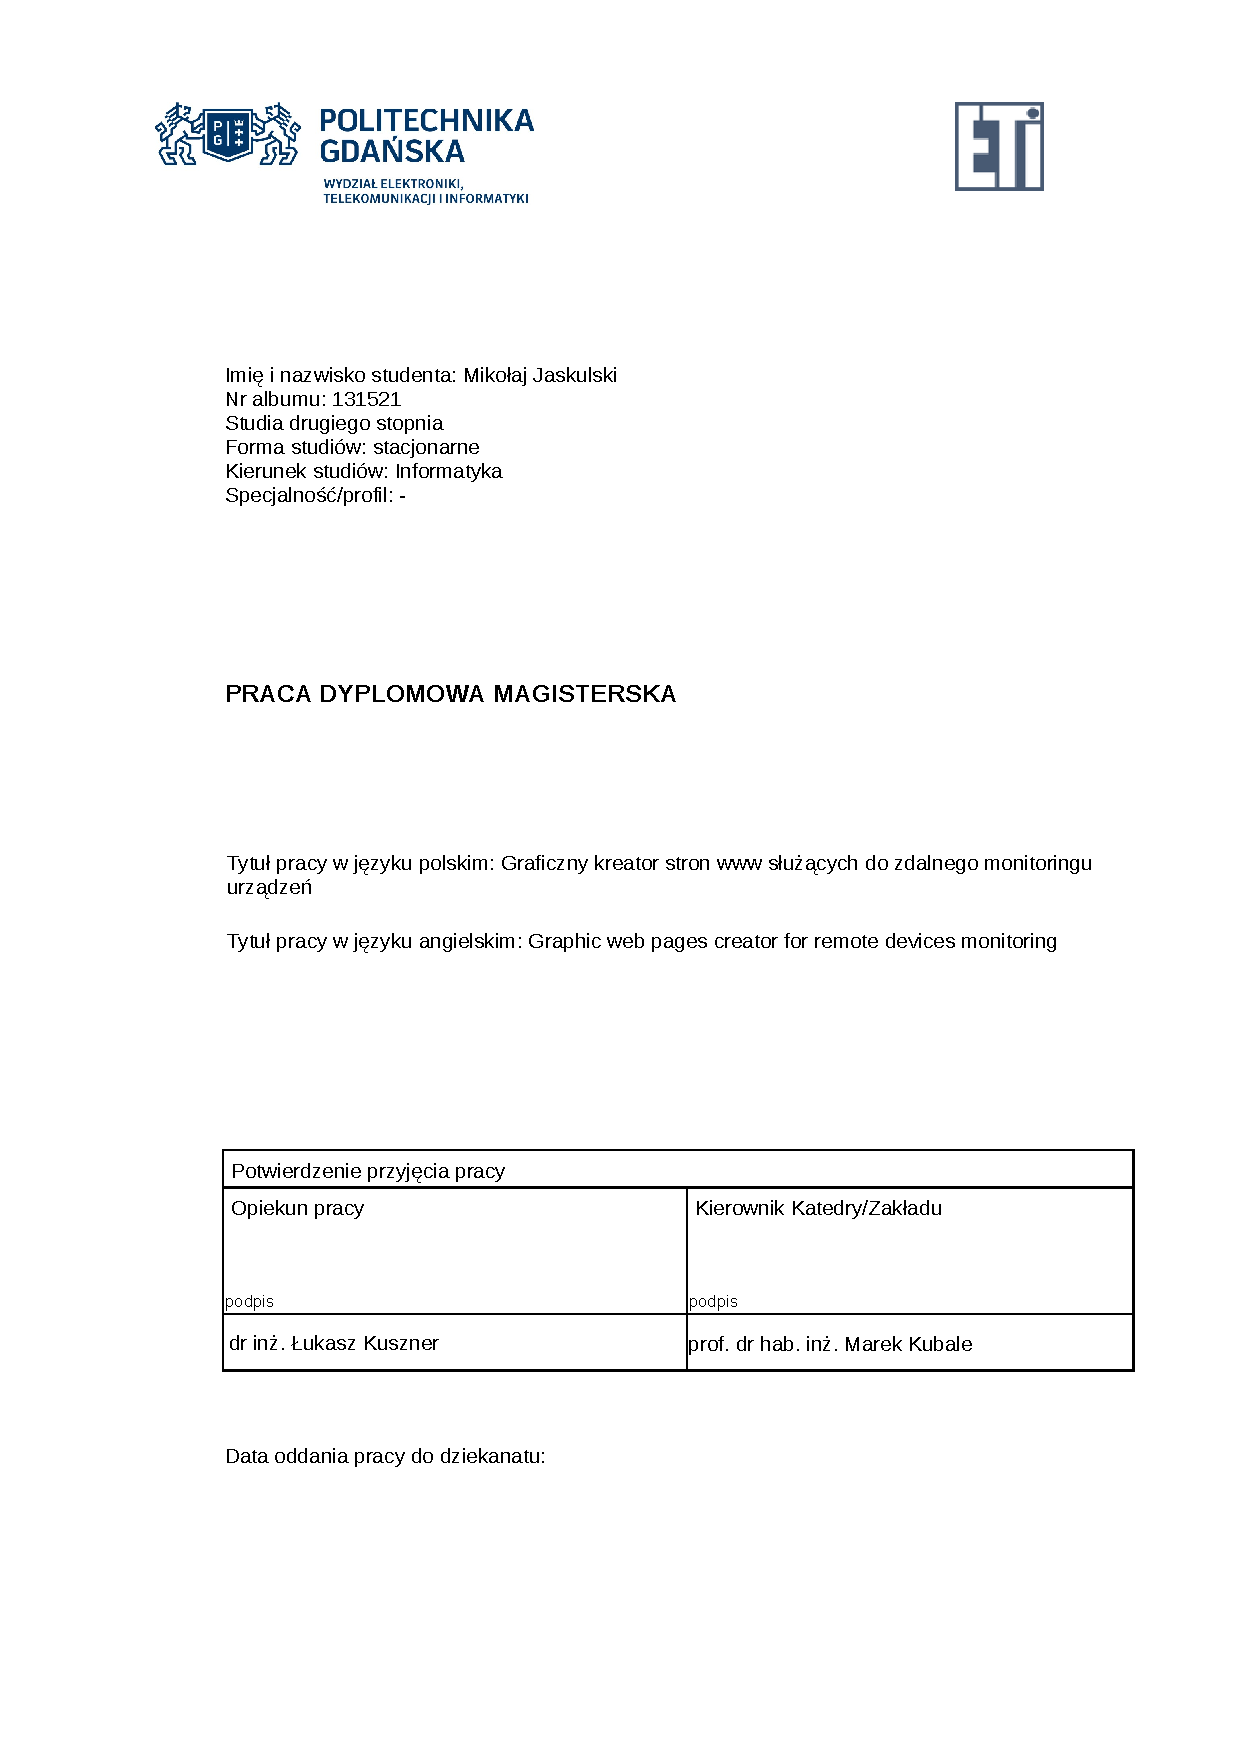
\includepdf{TitlePage.pdf}
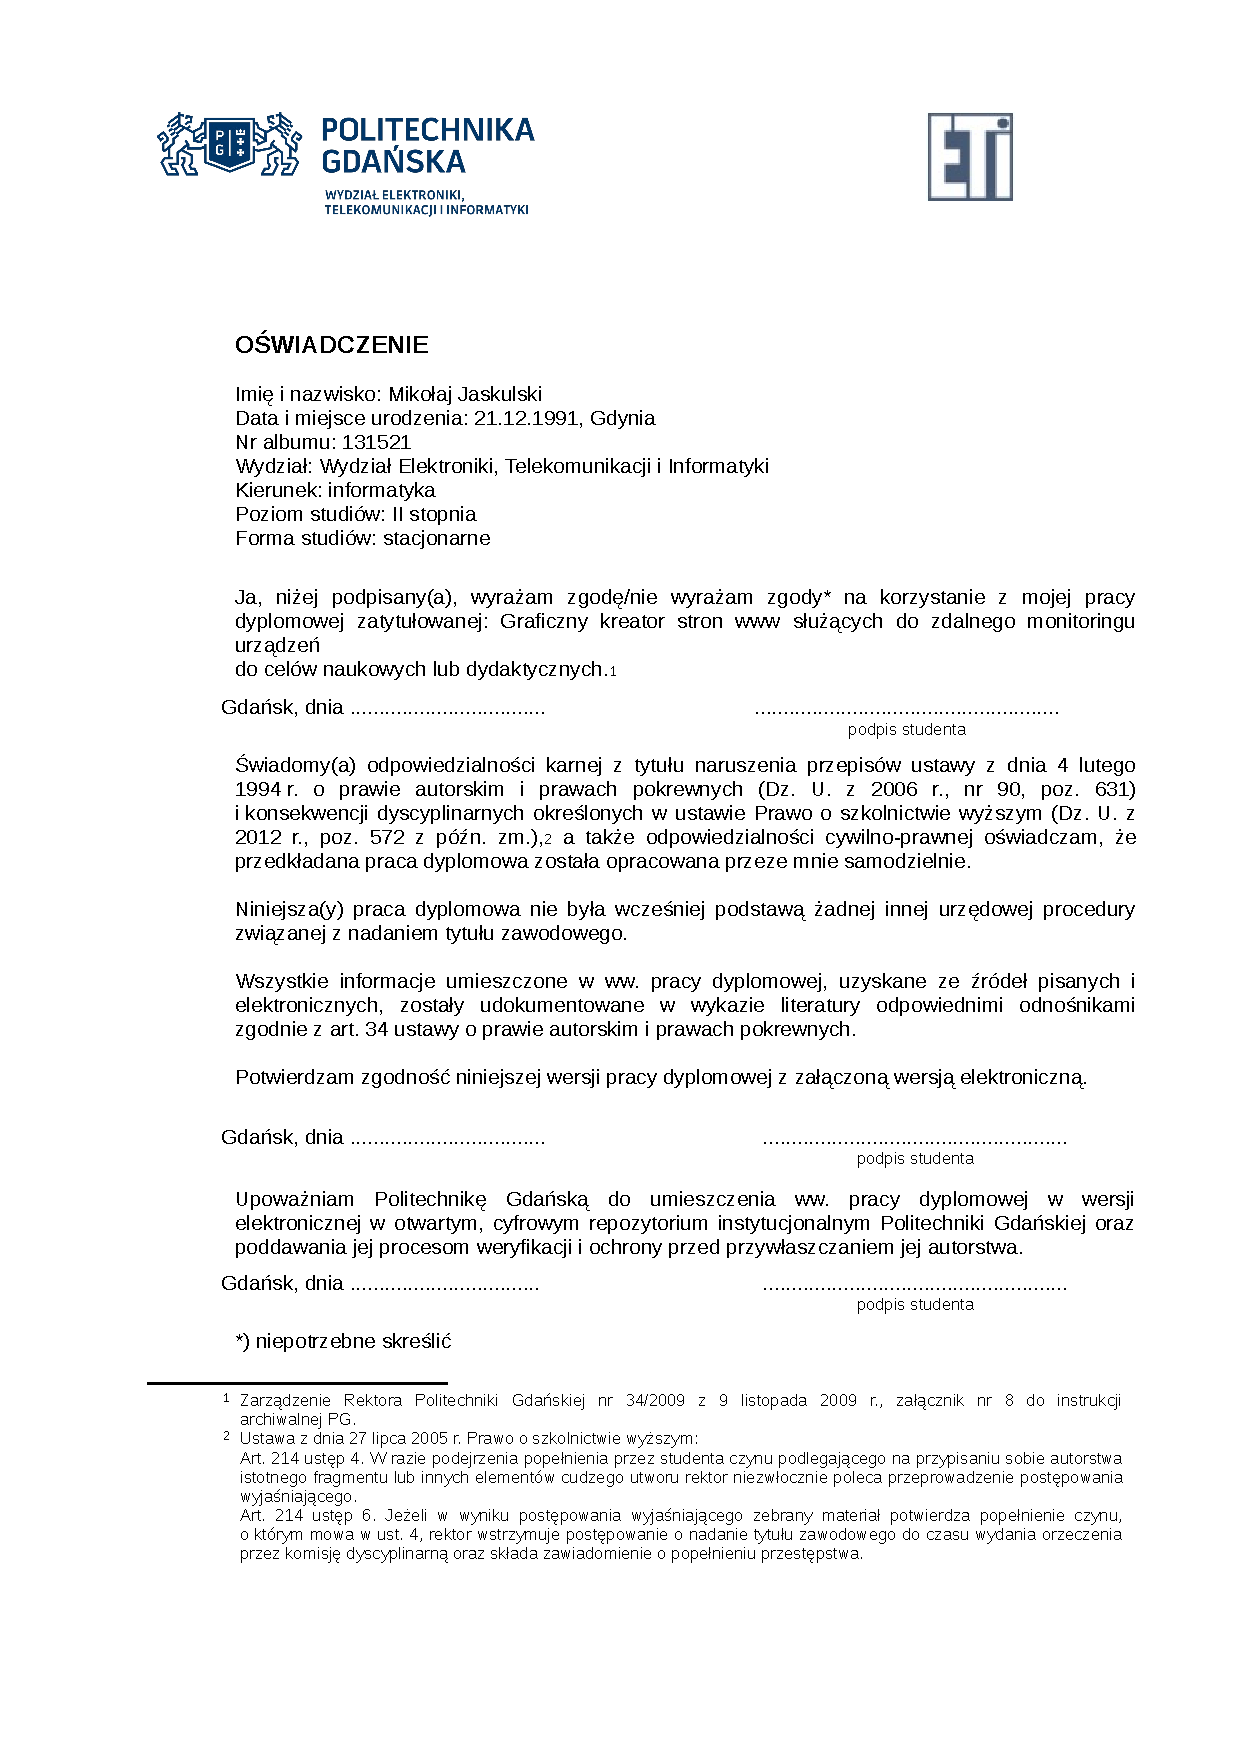
\includepdf{Statement.pdf}


\chapter*{Streszczenie}

Celem niniejszej pracy magisterskiej było stworzenie narzędzia, służącego do projektowania stron internetowych zawierających wizualizacje pracy urządzeń energetyki kolejowej. Narzędzie to zostało zaimplementowane jako aplikacja internetowa o nazwie Elements. Praca jest podzielona na pięć rozdziałów.

Pierwszy z nich zawiera opis systemu sterowania urządzeniami elektrycznego ogrzewania rozjazdów kolejowych. System zorganizowany jest w strukturę, w skład której wchodzą określone warstwy. Są nimi: warstwa urządzeń wykonawczych, autonomicznych rozdzielnic energetycznych, archiwizacji i obróbki danych, nadzoru i zarządzania oraz komunikacji. Każda z nich jest dokładnie opisana w odpowiednim podrozdziale. Szczególną uwagę poświęcono hierarchii urządzeń oraz komunikacji między nimi, gdyż miały one duży wpływ podczas tworzenia aplikacji.

Rozdział drugi opisuje proces wyboru technologii, za pomocą których została stworzona aplikacja. Wybór technologii back-endu był narzucony przez istniejące biblioteki wykonane w języku C\#, których użycie było konieczne do zrealizowania projektu. Wybór narzędzi służących do wykonania części front-end był trudniejszy z uwagi na dużą ilość istniejących rozwiązań do porównania. Rozdział zawiera ich analizę, porównanie oraz wyjaśnienie przyczyn wyboru jednej z nich. Wybrane technologie zostały szczegółowo opisane w rozdziale trzecim.

W rozdziale czwartym wyjaśniono w jaki sposób rozwiązanie zostało zaprojektowane. Aplikacja została nazwana Elements i podzielona na dwa moduły ze względu na ich odrębne funkcje. Pierwszy z nich - Designer służy do projektowania widoków z komponentów. Drugi, o nazwie Viewer, prezentuje wcześniej stworzone projekty użytkownikowi końcowemu.

Ostatni fragment pracy opisuje metody zastosowane do implementacji aplikacji. Opisane zostały jej składowe: warstwa serwera aplikacji jak i interfejsu użytkownika. Rozdział zawiera opis implementacji dwóch modułów, na które została podzielona aplikacja. Porusza również kwestię elementów reprezentujących zmienne urządzeń oraz mechanizm pobierania ich i prezentacji na stronie internetowej.

\chapter*{WSTĘP}

Celem niniejszej pracy magisterskiej było stworzenie narzędzia, służącego do projektowania stron internetowych zawierających wizualizacje pracy urządzeń energetyki kolejowej. Narzędzie to zostało zaimplementowane jako aplikacja internetowa o nazwie Elements. Praca jest podzielona na pięć rozdziałów.

Pierwszy z nich zawiera opis systemu sterowania urządzeniami elektrycznego ogrzewania rozjazdów kolejowych. System zorganizowany jest w strukturę, w skład której wchodzą określone warstwy. Są nimi: warstwa urządzeń wykonawczych, autonomicznych rozdzielnic energetycznych, archiwizacji i obróbki danych, nadzoru i zarządzania oraz komunikacji. Każda z nich jest dokładnie opisana w odpowiednim podrozdziale. Szczególną uwagę poświęcono hierarchii urządzeń oraz komunikacji między nimi, gdyż miały one duży wpływ podczas tworzenia aplikacji.

Rozdział drugi opisuje proces wyboru technologii, za pomocą których została stworzona aplikacja. Wybór technologii back-endu był narzucony przez istniejące biblioteki wykonane w języku C\#, których użycie było konieczne do zrealizowania projektu. Wybór narzędzi służących do wykonania części front-end był trudniejszy z uwagi na dużą ilość istniejących rozwiązań do porównania. Rozdział zawiera ich analizę, porównanie oraz wyjaśnienie przyczyn wyboru jednej z nich. Wybrane technologie zostały szczegółowo opisane w rozdziale trzecim.

W rozdziale czwartym wyjaśniono w jaki sposób rozwiązanie zostało zaprojektowane. Aplikacja została nazwana Elements i podzielona na dwa moduły ze względu na ich odrębne funkcje. Pierwszy z nich - Designer służy do projektowania widoków z komponentów. Drugi, o nazwie Viewer, prezentuje wcześniej stworzone projekty użytkownikowi końcowemu.

Ostatni fragment pracy opisuje metody zastosowane do implementacji aplikacji. Opisane zostały jej składowe: warstwa serwera aplikacji jak i interfejsu użytkownika. Rozdział zawiera opis implementacji dwóch modułów, na które została podzielona aplikacja. Porusza również kwestię elementów reprezentujących zmienne urządzeń oraz mechanizm pobierania ich i prezentacji na stronie internetowej.


\singlespacing
\tableofcontents
\onehalfspacing

\chapter{System DIMAC-EK}

Niniejsza praca magisterska związana jest bezpośrednio z systemem sterowania urządzeniami energetyki kolejowej o nazwie DIMAC-EK. Niniejszy rozdział zawiera pobieżny opis systemu, by przybliżyć czytelnikowi tematykę pracy.

\section{Funkcje}

System DIMAC-EK jest złożonym rozwiązaniem zajmującym się sterowaniem automatyką kolejową\cite{dimacek-katalog}. Jego głównym zadaniem jest zapewnienie drożności tras kolejowych podczas trudnych warunków pogodowych oraz dostarczanie pomiarów związanych z tą funkcją. Czynności te dotyczą głównie okresu zimowego, gdy mróz oraz śnieg jest w stanie blokować działanie rozjazdów kolejowych oraz tarasować przejazd. W skład systemu wchodzą następujące elementy:

\begin{itemize}
\item oświetlanie oraz osuszanie terenów kolejowych,
\item ochrona antywłamaniowa i przeciwpożarowa,
\item pomiar zużycia energii elektrycznej,
\item elektryczne ogrzewanie rozjazdu.
\end{itemize}

\section{Budowa}
Rozwiązanie będące przedmiotem niniejszej pracy ma bezpośredni związek z ostatnią funkcją systemu -- elektrycznym ogrzewaniem rozjazdów. Jest ono realizowane za pomocą grzałek elektrycznych montowanych na torach, które połączone są z urządzeniami nadzorującymi ich pracę \cite{dimacek-wytyczne}. Urządzenia dzielą się na dwie grupy. Pierwszą z nich są sterowniki, które kontrolują pracę grzałek na podstawie odczytów z przetworników pogodowych. Druga to urządzenia nadrzędne, które służą do zdalnego sterowania wszystkimi urządzeniami oraz gromadzenia i dalszego przesyłu danych dostarczanych przez nie. Dane te są archiwizowane przez serwer, co umożliwia ich późniejszą analizę.

Strukturę systemu przedstawia schemat \ref{fig:dimacek-scheme}.
\begin{figure}[h]
	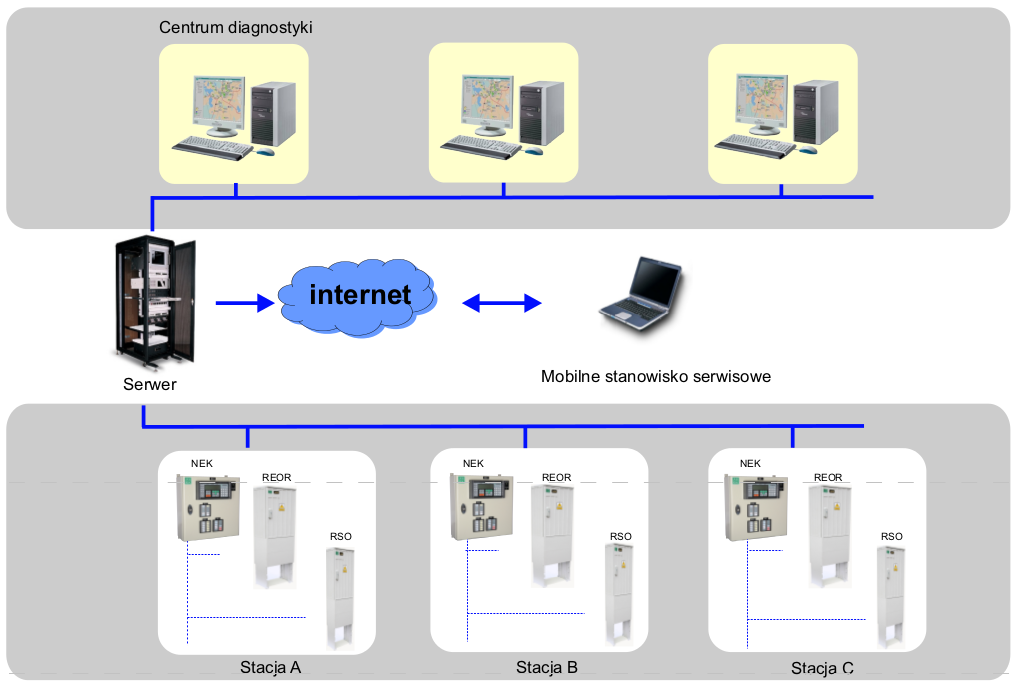
\includegraphics[height=85mm]{./img/dimacek_struktura.png}
	\caption[Struktura systemu DIMAC-EK]{Struktura systemu DIMAC-EK \cite{arex-materials}}
	\label{fig:dimacek-scheme}
\end{figure}

\section{Standard otwarty}
DIMAC-EK został wdrożony przez firmę Arex na zamówienie Polskich Lini Kolejowych. Najpierw na kilku stacjach, a następnie system został wdrożony w całym kraju. W związku z tym nastąpiła konieczność utworzenia otwartego standardu, który jasno określa wymogi dla dostarczanych przez firmy urządzeń grzewczych. Standard ten został nazwany Standardem KHA\cite{dimacek-wytyczne}. Każda firma produkująca sprzęt zgodny z KHA może być dostawcą urządzeń dla Polskich Kolei. Na kupno urządzeń oraz administrację systemu ogłaszane są okresowo przetargi.

\section{Struktura systemu}
System DIMAC-EK składa się z następujących warstw\cite{dimacek-wytyczne}:
\begin{itemize}
\item warstwa urządzeń pomiarowych -- przetworniki pogodowe,
\item warstwa urządzeń wykonawczych -- grzałki elektryczne,
\item warstwa autonomicznych rozdzielnic energetycznych -- rozdzielnice oraz sterowniki EOR,
\item warstwa archiwizacji i obróbki danych -- sterowniki nadrzędne NEK,
\item warstwa komunikacji systemu -- sieć GSM lub LAN,
\item warstwa nadzoru i zarządzania -- stanowiska diagnostyczne + serwer.
\end{itemize}


\subsection{Warstwa urządzeń pomiarowych}
Przetworniki zaopatrują sterowniki w dane pogodowe \cite{dimacek-wytyczne}. Jeden sterownik może odbierać dane z wielu przetworników. Dostępne są następujące typy przetworników pogodowych:
\begin{itemize}
\item temperatury powietrza,
\item prędkości wiatru,
\item detekcji deszczu (czujnik wilgoci),
\item detekcji śniegu,
\item temperatury szyny odniesienia (tzw. ,,zimnej''),
\item temperatury szyny ogrzewanej (tzw. ,,ciepłej''),
\item detekcji śniegu nawiewanego na rozjazd.
\end{itemize}

\subsection{Warstwa urządzeń wykonawczych}
Grzejniki można podzielić ze względu na sposób i miejsce ich montażu na torach oraz na moc. Wszystkie parametry grzejników dopuszczonych do użycia na torach znaleźć można w dokumentacji systemu dostarczanej przez PLK.


\subsection{Warstwa autonomicznych rozdzielnic energetycznych}
Rozdzielnice RESO przeznaczone są do sterowania obwodami elektrycznego ogrzewania rozjazdów oraz obwodami oświetleniowymi \cite{dimacek-wytyczne}. Poza funkcją sterującą dokonują one diagnostyki obwodów oraz przetworników pomiarowych. Można o nich myśleć jako o zbiorze współpracujących ze sobą urządzeń zamontowanych w jednym miejscu. Rozdzielnice zawierają sterowniki EOR oraz moduły sterująco-diagnostyczne, które sterują pracą grzałek. Sterowniki współpracują z urządzeniami nadrzędnymi NEK, dzięki czemu pracę rozdzielnicy RESO można kontrolować z poziomu zdalnych stanowisk dyspozytorskich.

\begin{figure}[t]
	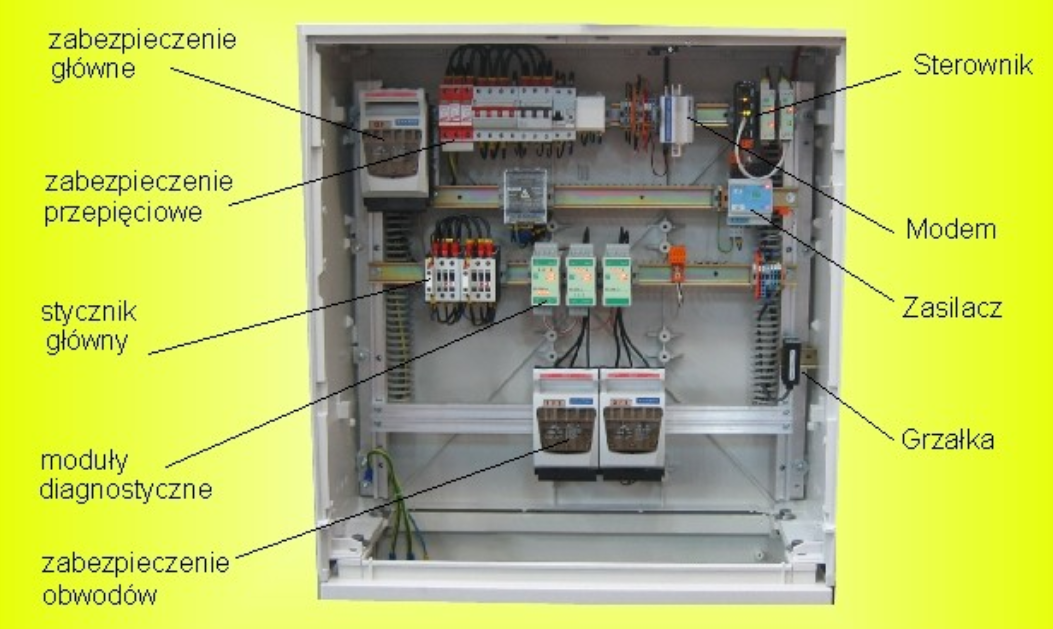
\includegraphics[height=95mm]{./img/dimacek_rozdzielnica.png}
	\caption[Budowa rozdzielnicy RESO]{Budowa rozdzielnicy RESO \cite{arex-materials}}
	\label{fig:dimacek-reso}
\end{figure}

Rozdzielnice mogą pełnić różne funkcje w zależności od umieszczonych w nich urządzeń. Urządzenia firmy Arex są elastyczne w swej konfiguracji i działają współpracując ze sobą lub nie. Na przykład, możliwe jest poprawne działanie sterowników grzałek bez integracji z modułami diagnostycznymi, służącymi do gromadzenia oraz przesyłu danych. Dzięki standardowi KHA, w rozdzielnicy można łączyć ze sobą różne rodzaje urządzeń wyprodukowanych przez różne firmy. Wygląd oraz zawartość rozdzielnicy można zobaczyć na zdjęciu \ref{fig:dimacek-reso}.

\subsection{Warstwa archiwizacji i obróbki danych}
Sterownik nadrzędny NEK służy do zdalnego monitorowania urządzeń systemu DIMAC-EK \cite{dimacek-wytyczne}. Umożliwia on również zdalne sterowanie wszystkimi podłączonymi do niego sterownikami z poziomu jednej stacji kolejowej. Dane gromadzone przez sterownik zapisywane są w jego wewnętrznej bazie danych, którą można zarządzać z jego poziomu. Możliwy jest również przesył danych w czasie rzeczywistym do serwera przez sieć Internet. Aby zapewnić elastyczność w dostępie do danych, urządzenie NEK posiada popularne interfejsy transmisyjne:
\begin{itemize}
\item konwerter RS232-TCP/IP,
\item modem GRPS,
\item modem telefoniczny.
\end{itemize}

\subsection{Warstwa komunikacji systemu}
W granicach stacji kolejowej urządzenia komunikują się z nadrzędnym sterownikiem w standardzie CAN/DIMNET-P4\cite{dimacek-wytyczne}.
Komunikacja pomiędzy sterownikami nadrzędnymi (NEK), a serwerami realizowana jest w oparciu o sieć intranet poprzez protokół DIMNET-P5. DIMNET-P5 jest autorskim rozwiązaniem firmy Arex, który został ustanowiony otwartym standardem komunikacji pomiędzy urządzeniami energetyki kolejowej przez Polskie Linie Kolejowe. Protokół ten można stosować przy użyciu dowolnego medium danych, lecz w praktyce stosuje się sieć Internet. Schemat struktury urządzeń systemu DIMAC-EK w sieci IP znajduje się na schemacie \ref{fig:dimacek_ip}.


\begin{figure}[t]
	\centerline{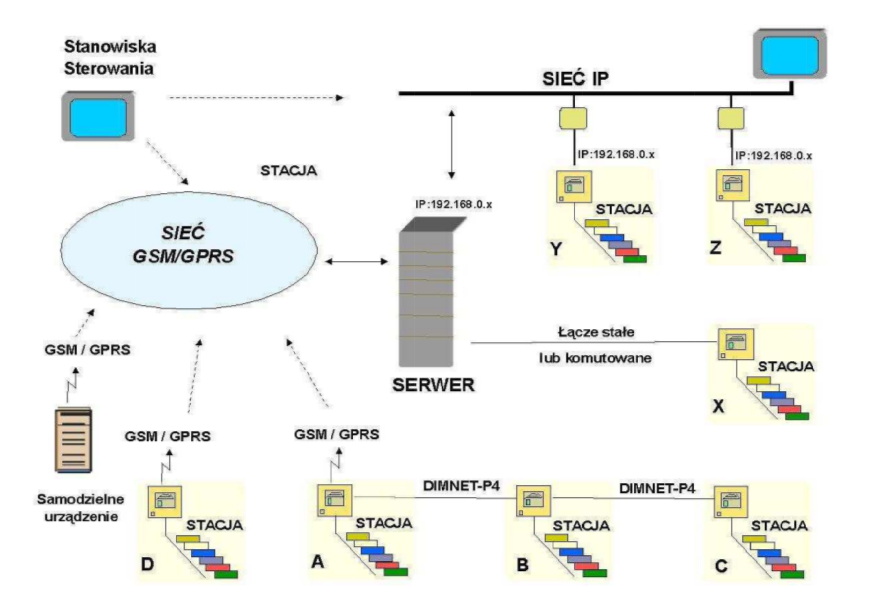
\includegraphics[height=125mm]{./img/dimacek_ip.png}}
	\caption[DIMAC-EK w sieci IP]{DIMAC-EK w sieci IP \cite{arex-materials}}
	\label{fig:dimacek_ip}
\end{figure}


\subsection{Warstwa nadzoru i zarządzania}

Dane przesłane przez wszystkie sterowniki nadrzędne NEK gromadzone są przez serwer danych w celu archiwizacji. Ostatnim elementem systemu jest aplikacja DIVIS. Służy ona do prezentacji zgromadzonych danych w sposób zrozumiały dla osób niemających wiedzy o budowie oraz działaniu urządzeń. Aplikacja dostarcza następujące informacje:


\begin{itemize}
\item dane pogodowe w przestrzeni czasu,
\item czas pracy grzałek,
\item energia zużyta podczas pracy grzałek oraz jej koszt,
\item dane dotyczące alarmów przeciwwłamaniowych oraz przeciwpożarowych,
\item statystyka oraz analiza powyższych danych.
\end{itemize}

Należy zwrócić uwagę, iż nie ma obecnie w systemie aplikacji dającej możliwość odbioru danych z urządzeń w czasie rzeczywistym.

Rozmieszczenie elementów wszystkich warstw na stacji kolejowej zobrazowane jest na schemacie \ref{fig:dimacek-scheme}.

\begin{figure}[t]
	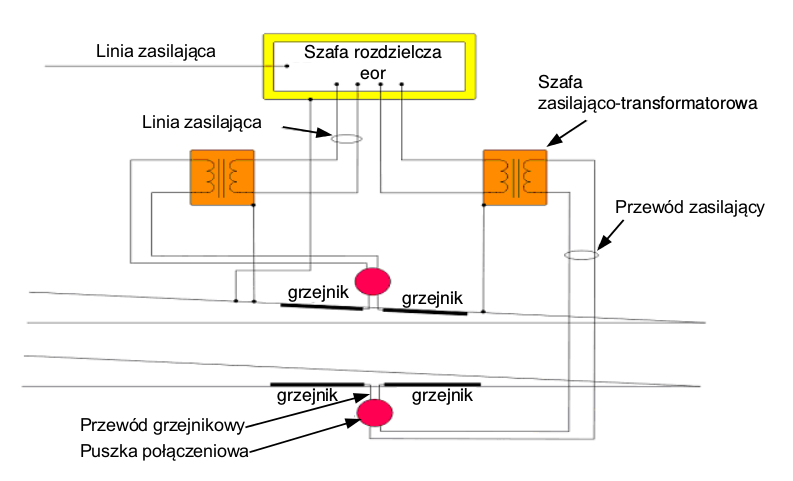
\includegraphics[height=85mm]{./img/dimacek_tory.png}
	\caption[Elementy systemu DIMAC-EK na stacji kolejowej]{Elementy systemu DIMAC-EK na stacji kolejowej \cite{arex-materials}}
	\label{fig:dimacek_tory}
\end{figure}

\section{DIMNET-P5 -- protokół komunikacji}
Jednym z większych problemów w budowie systemu monitorowania ogrzewania szyn kolejowych, są duże odległości między obiektami oraz całkowity brak towarzyszącej im infrastruktury komunikacyjnej \cite{dimnetp5-spec}. Do czasu udostępnienia telefonicznych sieci komórkowych, techniczne możliwości monitorowania instalacji ogrzewania rozjazdów kolejowych stacji były znacznie ograniczone. W związku z tym, firma Arex zapoczątkowała eksperymenty nad przesyłem danych między urządzeniami za pomocą sieci GSM w 2002 roku. Jako że w tym okresie przesyłanie pakietów danych przez sieć GSM nie było tanie, należało skupić się na tym, aby metoda przesyłu była jak najbardziej oszczędna. Rozwiązaniem tego problemu jest protokół komunikacji o nazwie DIMNET-P5.

\subsection{Warstwy protokołu}
DIMNET-P5 oparty jest na wzorcu podziału usług protokołu na warstwy zgodnie z zaleceniami 7-warstwowego modelu referencyjnego ISO-OSI IEC7498 \cite{dimnetp5-spec}. W ramach protokołu zdefiniowane są jedynie warstwy powyżej transportowej (4 wg. ISO/OSI), gdyż DIMNET-P5 bazuje na powszechnie stosowanym w sieciach stosie protokołów TCP/IP i korzysta z usług protokołu TCP. Powyższymi warstwami są:
\begin{itemize}
\item warstwa kodowania -- służy do wydzielania datagramów z niezawodnych strumieni bajtów w połączeniach TCP. Może również realizować opcjonalne formy kodowania lub zabezpieczania integralności danych (obsługa sum kontrolnych CRC),
\item warstwa sesji -- odpowiedzialna za nawiązywanie połączenia i utrzymywanie nad nim kontroli oraz realizację wirtualnych kanałów transmisji do urządzeń w ramach jednego połączenia,
\item warstwa aplikacji -- realizuje usługi komunikacyjne dostępne dla programów aplikacyjnych w stacjach końcowych.
\end{itemize}

\subsection{Jednostki i typy danych}
Urządzenia w standardzie DIMNET-P5 prezentowane są jako uporządkowany zbiór jednostek danych. Każda jednostka posiada przypisany jednoznaczny indeks, za pomocą którego identyfikowana jest zmienna \cite{dimnetp5-spec}. Każda jednostka ma również przyporządkowany typ danych. Dopuszczalne typy danych są następujące:
\begin{itemize}
\item liczba całkowita ze znakiem lub bez (8, 16, 32, 64 bity),
\item liczba zmiennoprzecinkowa (8, 16, 32, 64 bity),
\item ciąg znaków kodowanych za pomocą ASCII o określonej długości.
\end{itemize}

\subsection{Model komunikacji}
Komunikacja w DIMNET-P5 odbywa się najczęściej pomiędzy urządzeniami zdalnymi (sterownikami kontrolującymi grzałki) oraz sterownikami nadrzędnymi (NEK, serwery danych) \cite{dimnetp5-spec}. Aby zrozumieć sposób komunikacji między stacjami końcowymi należy poznać podstawy komunikacyjne w DIMNET-P5. Określają one podstawowe interakcje występujące pomiędzy programem aplikacyjnym, a warstwą aplikacji. Są to:
\begin{itemize}
\item request -- wysłanie inicjujące, wysłanie danych lub żądania obsługi,
\item indication -- odbiór danych lub żądania obsługi,
\item response -- wysłanie odpowiedzi na wcześniejsze żądanie obsługi,
\item confirmation -- odbiór odpowiedzi potwierdzający realizację żądania.
\end{itemize}


W standardzie DIMNET-P5 możliwe są trzy sposoby komunikacji opisane poniżej.
\begin{itemize}
\item Relacja klient serwer -- relacja pomiędzy pojedynczym klientem i pojedynczym serwerem. Standardowa relacja typu żądanie -- odpowiedź.
\item Relacja producent-konsument -- relacja między pojedynczym producentem i pojedynczym konsumentem. Producent generuje w asynchroniczny sposób komunikaty z danymi, które nie wymagają potwierdzenia. Relacja nie określa jak często lub w jakich przypadkach następuje wysłanie komunikatu.
\item Super-relacja klient-serwer -- rozpoczynana przez polecenie uruchomienia procesu. Stacja, która jest serwerem potwierdza odpowiednim sygnałem sukcesu lub porażki uruchomienie procesu. W przypadku gdy odpowiedź jest pozytywna, relacja przechodzi do typu producent-konsument. Konsumentem staje się stacja typu serwer. Odstęp czasowy pomiędzy komunikatami są regulowane w całości przez proces. Polecenie zakończenia procesu powinna wysłać stacja klienta. Stacja serwer w tej sytuacji odsyła potwierdzenie otrzymania komunikatu i zatrzymuje proces. Relacja ta jest zobrazowana na schemacie \ref{fig:dimnetp5}.

	\begin{figure}[t]
		\centerline{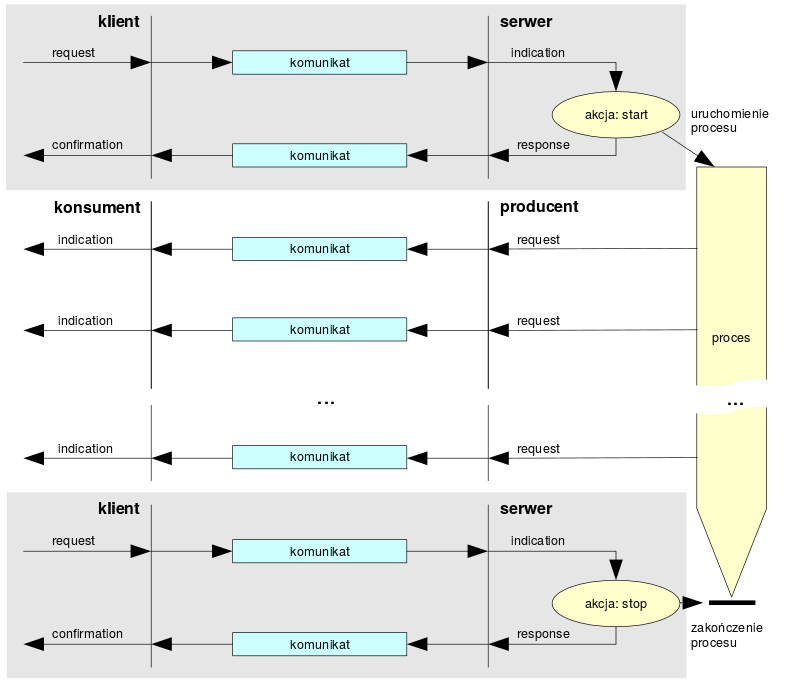
\includegraphics[height=125mm]{./img/dimnet-p5.png}}
		\caption[Super-relacja serwer-klient]{Super-relacja serwer-klient \cite{arex-materials}}
		\label{fig:dimnetp5}
	\end{figure}
\end{itemize}

\subsection{Przykład zastosowania w systemie DIMAC-EK}
W systemie DIMAC-EK super-relację klient-serwer implementują na przykład\cite{dimacek-wytyczne}:
\begin{itemize}
\item serwer gromadzący dane, który jest klientem połączenia,
\item sterownik nadrzędny NEK, który pełni funkcję serwera.
\end{itemize} 
Serwer danych inicjuje połączenie, a następnie odbiera paczki z danymi od urządzenia. NEK wysyła pakiety z danymi nieustannie, do momentu sygnału zakończenia połączenia wysłanego przez serwer. Taka organizacja ma dwie podstawowe zalety: brak konieczności ciągłego odpytywania danych przez klienta oraz wysyłanie paczki danych jedynie wtedy, gdy nowe wartości różnią się od poprzednich.

\subsection{Sterowanie połączeniem}
Standard DIMNET-P5 umożliwia dodatkowe czynności sterujące połączeniem, przydatne w wielu sytuacjach. Poniżej znajduje się ich opis.
\begin{itemize}
\item Logowanie -- Proces logowania jest pierwszą czynnością, która powinna zostać zapoczątkowana przez klienta nawiązującego połączenie z serwerem. Bez zakończenia tej czynności powodzeniem, stacja klienta ani serwera nie mogą wymieniać się żadnymi danymi. Podczas logowania następuje wymiana zakodowanego klucza dostępu.
\item Wylogowanie -- czynność kończąca połączenie na podstawie żądania którejś ze stron połączenia. Wylogowanie może nastąpić w skutek zbyt długiego oczekiwania na pakiet utrzymujący połączenie. W takim wypadku łączność uznaje się za przerwaną.
\item Kontrola połączenia -- polega na okresowej wymianie między stacjami datagramu utrzymującego połączenie, tzw. heartbeatu.
\item Synchronizacja czasu -- dokonuje się jej przez datagram heartbeat. Polega na dołączeniu przez klienta do heartbeatu żądania synchronizacji. Serwer po odebraniu żądania, dołączy swój czas do kolejnego datagramu heartbeatu wysyłanego przez siebie.
\end{itemize}


\section{System Monitorowanie Urządzeń Energetycznych}
Ostatnim elementem systemu DIMAC-EK jest platforma SMUE -- System Monitoringu Urządzeń Energetycznych stworzona przez firmę Arex. Jest to rozwiązanie, które współpracuje z serwerem danych archiwalnych urządzeń\cite{dimacek-wytyczne}. 

\subsection{Przyczyny powstania systemu}
W wielu przypadkach, po wdrożeniu systemu zdalnego monitoringu urządzeń na stacji, błędy w działaniu systemu uwidaczniały się dopiero po sezonie grzewczym \cite{dimacek-wytyczne}. Przyczyny problemów były następujące:
\begin{itemize}
\item nieumiejętna obsługa urządzeń,
\item awarie mechaniczne urządzeń,
\item kradzieże i zniszczenia,
\item problemy na drodze komunikacji.
\end{itemize}

Aby szybko reagować na powyższe sytuacje, stworzony została aplikacja SMUE.

\subsection{Opis aplikacji}
SMUE jest aplikacją internetową przeznaczoną dla osób, które nie muszą posiadać zaawansowanej wiedzy technicznej dotyczącej urządzeń oraz branży kolejowej\cite{dimacek-wytyczne}. Służy ona do prezentacji danych pomiarowych oraz dotyczących różnych zdarzeń przesyłanych z urządzeń zainstalowanych w terenie. SMUE analizuje je, dokonuje statystyki oraz analizy i prezentuje użytkownikowi w przejrzysty sposób. Dane gromadzone są  przez serwer i archiwizowane w bazie danych. Przykładowa strona z raportem znajduje się na obrazie \ref{fig:smue}.\\

\begin{figure}[h]
		\centerline{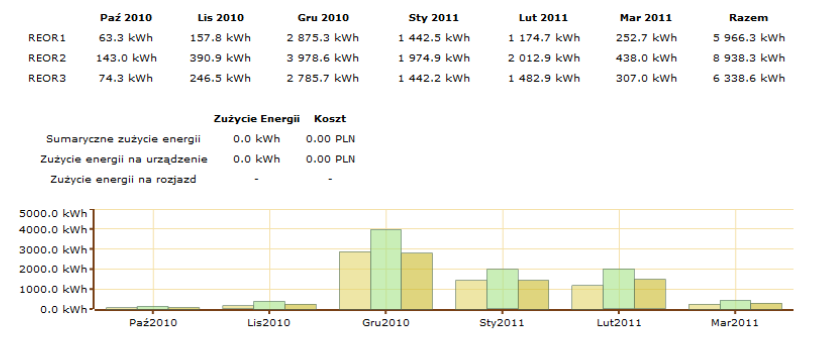
\includegraphics[height=75mm]{./img/smue.png}}
		\caption{Zestawienie zużycia energii elektrycznej w aplikacji SMUE}
		\label{fig:smue}
\end{figure}

SMUE dostarcza następujące informacje:
\begin{itemize}
\item archiwalne pomiary pogodowe (temp. powietrza, wilgotność, opady atmosferyczne),
\item raporty dotyczące zużycia energii elektrycznej w różnych okresach czasu,
\item porównania dotyczące różnych stacji kolejowych na podstawie wybranych danych,
\item tabela zdarzeń urządzeń (rozpoczęcie, zakończenie grzania, włamania, utrata połączenia, usterki).
\end{itemize}

\section{Podsumowanie}
System DIMAC-EK jest kompletnym systemem służącym do monitorowania urządzeń energetyki kolejowej. Posiada wszelkie możliwe komponenty do komunikowania, kontrolowania oraz diagnozowania urządzeń. Rozwiązanie zawiera również narzędzie do analizowania danych zbieranych przez system. Warto jednak zauważyć, iż nie istnieje rozwiązanie, które byłoby w stanie zaprezentować w przejrzysty sposób dane z urządzeń w czasie rzeczywistym. Praktyczna część niniejszej pracy została poświęcona temu problemowi.
\chapter{Architektura aplikacji oraz wybór technologii}

Rozdział ten zawiera opis architektury oraz metodyk, które zostały użyte do wykonania zadania. W rozdziale przedstawiono również wady oraz zalety technologii, których użycie było brane pod wagę do realizacji projektu. Ilość dostępnych technologii oraz narzędzi sprawia, iż wybranie najbardziej odpowiedniej z nich do określonego celu nie było prostym zadaniem.

\section{Projekt architektury aplikacji}
Jedno z wymagań projektu stanowi o tym, iż rozwiązanie ma być dostępne dla użytkowników z poziomu przeglądarki internetowej. Projekt zostanie zatem zrealizowany jako aplikacja internetowa. Kolejną cechą aplikacji będzie posiadanie złożonego interfejsu użytkownika umożliwiającego projektowanie wizualizacji pracy urządzeń. Uzasadnione w tym przypadku jest rozdzielenie projektu aplikacji na dwie warstwy: back-end oraz front-end w celu modularyzacji rozwiązania. 

\subsection{Warstwa front-end}
Jednym z głównych zadań interfejsu jest prezentowanie stanu aplikacji użytkownikowi. Warstwa ta nie będzie posiadać logiki biznesowej, wszelkie potrzebne dane dotyczące jej zostaną pobrane z serwera.

\subsection{Warstwa back-end}
Głównymi zadaniami warstwy back-end będą:
\begin{itemize}
\item wykonywanie logiki biznesowej i przekazywanie jej rezultatów do warstwy interfejsu,
\item gromadzenie i przechowywanie odpowiednich danych wymaganych do działania aplikacji.
\end{itemize}

Jako że stan aplikacji będzie przechowywany przez interfejs użytkownika, nie ma konieczności aby funkcjonalność tę realizował równolegle back-end. Warstwa ta zostanie zatem zrealizowana w postaci usług sieciowych w architekturze REST. Podstawowym założeniem architektury REST jest bezstanowość podczas realizacji funkcjonalności\cite{rest-book} i dlatego właśnie ta metoda została wybrana do realizacji zadania.

\subsection{Testowanie}
Podczas realizacji projektu zostaną użyte testy jednostkowe. Testowanie komponentów składowych aplikacji w trakcie tworzenia funkcjonalności posiada wiele zalet. Są nimi między innymi\cite{tests-book}:
\begin{itemize}
\item zwiększenie modularyzacji aplikacji,
\item zmniejszenie zależności między komponentami,
\item wymuszenie większej uwagi podczas tworzenia komponentów,
\item stworzone testy są elementem dokumentacji kodu.
\end{itemize}

W oparciu o testy jednostkowe powstała metodyka wytwarzania oprogramowania, tzw. Test Driven Development (TDD)\cite{tests-book}. Wymusza ona na programiście pisanie testu zanim jeszcze powstanie komponent. Głównym zadaniem tej metodyki jest lepsze zrozumienie funkcji tworzonego przez programistę komponentu. 
Metodyka TDD zostanie zastosowana podczas tworzenia aplikacji.

\section{Wybór technologii Back-end}

Zadanie nieco ułatwił fakt, iż podczas realizacji projektu było dostępne rozwiązanie do komunikacji z serwerem urządzeń. Była nim biblioteka wykonana w języku C\#. Aby bez trudu skorzystać z jej wszystkich możliwości do stworzenia backendowej części aplikacji posłużono się językiem C\# oraz frameworkiem pozwalającym na szybkie tworzenie aplikacji internetowych MVC4. Framework ten został wybrany z następujących powodów\cite{mvc-book}:

\begin{itemize}
\item jest najnowszym frameworkiem do tworzenia aplikacji internetowych rozwijanym przez firmę Microsoft, która posiada wieloletnie doświadczenie w dostarczaniu rozwiązań dla programistów,
\item pozwala na pełną kontrolę nad dynamicznie generowaną treścią strony,
\item jest zgodny z metodyką Test Driven Development,
\item łatwo integruje się z JavaScript,
\item pozwala na szybkie tworzenie usług typu RESTful.
\end{itemize}


\section{Wybór technologii Front-end}

W przeciwieństwie do technologii aplikacji po stronie serwera, wybór odpowiedniego narzędzia do stworzenia dynamicznego interfejsu aplikacji internetowej był trudniejszym zadaniem niż wybór technologii backendowej. Z obecnie stosowanych do tego celu rozwiązań najczęściej stosuje się technologię wspieraną przez każdą współczesną przeglądarkę -- JavaScript\cite{javascript-book} (przyczyny takiego stanu rzeczy opisane są szczegółowo w rozdziale 3). Na tym zadanie wyboru się nie kończy. Wynika to z faktu, iż JavaScript jest technologią w której trudno zachować logiczną strukturę projektu. Dowodem na to jest powstanie dużej ilości frameworków. Istnieje nawet strona internetowa, która pozwala na dobranie odpowiedniego narzędzia do potrzeb projektu spośród 78\cite{todomvc}. Każdy z nich rozwiązuje jednak problem tworzenia bogatego interfejsu aplikacji internetowej w inny sposób. Często wybieraną formą organizacji projektu narzucaną przez frameworki jest implementacja wzorca projektowego Model View Controller. Jako że nie jest to w przypadku JavaScript łatwe zadanie, każdy framework realizuje wzorzec na swój sposób, ,,rozmywając'' zakres obowiązków poszczególnych składowych MVC. Z tego powodu powstały terminy określające, rodzinę farmeworków JavaScript -- MV*, i MVW (\textit{Model, View, Whatever}). 

Aby wytypować rozwiązanie, które będzie najbardziej pomocne w realizacji projektu należy dokonać analizy posługiwania się nim. Jest to skuteczny sposób aby wytypować framework, który najłatwiej zaadaptuje się do określonej sytuacji\cite{todomvc}. Poprzez próbę użycia go można stwierdzić czy nada się on do rozwiązywanego problemu. 
W poniższych podrozdziałach przedstawione zostały najbardziej popularne na tę porę rozwiązania służące do tworzenia bogatego interfejsu aplikacji internetowych. Każdemu z nich przypisano również kilka cech, które są równie istotne podczas wybierania narzędzia organizującego projekt. Są nimi:
\begin{itemize}
\item dojrzałość rozwiązania,
\item rozmiar społeczności związanej z rozwiązaniem,
\item określenie w jakich dużych projektach rozwiązanie zostało wdrożone,
\item rozmiar rozwiązania.
\end{itemize}

\section{AngularJS}

AngularJS jest frameworkiem stworzonym przez firmę Google w 2010 roku \cite{angular-book}. Narzuca on użycie wzorca projektowego MVVM -- Model, View, ViewModel, które są głównymi elementami tworzonymi przez programistę podczas tworzenia aplikacji za pomocą frameworku. 

\subsection{Widoki i dyrektywy}
AngularJS wyróżnia się z pośród innych frameworków tym, iż umożliwia wykorzystanie dodatkowych elementów rozszerzających HTML zwanych dyrektywami \cite{angular-book}. Można o nich myśleć jak o dodatkowych atrybutach węzłów HTML, które zaczynają się od znaków \textit{ng-}. Dyrektywy mają różne zastosowanie. Można wyróżnić między innymi dyrektywy służące do:
\begin{itemize}
\item powiązań (binding) między widokiem, a modelem i kontrolerem -- np. \textit{ng-model}, \textit{ng-binding}, \textit{ng-controler},
\item tworzenia prostej logiki generowania dynamicznych elementów strony -- np. \textit{ng-repeat},
\item reagowania na zdarzenia -- np. \textit{ng-click}.
\end{itemize}

Oprócz dyrektyw istnieje jeszcze jedno dodatkowe wyrażenie służące do powiązania zmiennej kontrolera z odpowiadającą jej zmienną widoku. Służy do tego podwójny nawias klamrowy, tzw. znacznik. Gdy odpowiadająca mu zmienna kontrolera zmieni swoją wartość, węzeł HTML zawierający znacznik zostanie odświeżony.

Poniżej znajduje się przykład wykorzystania dyrektyw wraz ze znacznikiem:

\begin{lstlisting}[language=HTML5]
<body ng-app='bmiApp'>
  <div ng-controller='bmiController as bmi'>
   <div>
       Wzrost: <input type="number" ng-model="wzrost">
     </div>
     <div>
       Waga: <input type="number" ng-model="waga">
     </div>
     <div>
       Wynik: {{wzrost / (waga * waga)}}
     </div>
     <button ng-click='bmi.pokazBMI()'>Pokaz wynik</button>
  </div>
</body>
\end{lstlisting}

Pliki zawierające dyrektywy noszą nazwę szablonu (template) oraz muszą być skompilowane przez kompilator AngularJS przed umieszczeniem ich na serwerze aplikacji.

\subsection{Kontroler}
Kontrolery są obiektami JavaScript które, zawierają logikę interfejsu \cite{angular-book}. Ich zadanie nie różni się od klasycznego kontrolera z wzorca MVC. Są tworzone po to, by przygotować obiekty Modelu i następnie przekazać je do Widoku. Kontrolery tworzy się za pomocą metody \textit{controller} obiektu \textit{angular}. Przykładowy kontroler reagujący na zmianę pól tekstowych input oraz wyświetlający wynik dodawania wprowadzonych liczb w ostatnim węźle div znajduje się poniżej:

\begin{lstlisting}[language=JavaScript]
angular.module('bmi', [])
.controller('BmiController', function() {
  this.wzrost = 180;
  this.waga = 70;

  this.pokazBMI = function() {
  	bmi = this.wzrost / ( this.waga * this.waga);
    window.alert(bmi);
  };
});
\end{lstlisting}


\subsection{Usługa}
Usługi są obiektami, które powinny zawierać logikę biznesową -- wszelkie nie związane bezpośrednio z działaniem interfejsu. Do tworzenia usługi służy metoda \textit{factory} obiektu \textit{angular}. Należy nadać jej nazwę analogicznie jak w przypadku kontrolera. Przykładowe stworzenie usługi może wyglądać następująco:
\begin{lstlisting}[language=JavaScript]
angular.module('bmiServiceModule', [])
.factory('bmiService', function() {
	this.pokazBMI = /* cialo metody */
});
\end{lstlisting}

Aby powiązać kontroler kalkulatora z usługą, należy przekazać jej nazwę do metody \textit{controller} obiektu \textit{angular} w taki sposób:
\begin{lstlisting}[language=JavaScript]
angular.module('bmi', ['bmiServiceModule'])
.controller('BmiController', ['bmiService', function(bmiService) {
	this.pokazBMI = function(){
		bmiService.pokazBMI();
	}
}]);
\end{lstlisting}

\section{BackboneJS}
BackboneJS jest frameworkiem który organizuje strukturę projektu JavaScript wykorzystując pojęcia Widoków oraz Modeli z wzorca MVC \cite{backbonejs}. BackboneJS umożliwia również deklarowanie oraz obsługę zdarzeń. Kolejną zaletą jest łatwa integracja rozwiązania z usługami sieciowymi typu RESTful. Korzystanie z frameworku w większej mierze opiera się na tworzeniu obiektów za pomocą klasy \textit{Backbone}.

\subsection{Modele}
Modele tworzy się używając metody \textit{extend} klasy \textit{Model}, która w konstruktorze przyjmuje strukturę typu klucz-wartość. Utworzony obiekt będzie posiadał pola o nazwach odpowiadającym kluczom, i przypisane do nich wartości. Wartością może być też funkcja. 
Model posiada również metody pozwalające na modyfikację oraz odczyt każdego z pól. Obiekty modelu można rozszerzać o obsługę zdarzeń. Dla przykładu, możliwe jest zdefiniowanie metody, która zostanie wywołana gdy wartość któregoś z pól obiektu modelu zmieni się. 
Poniżej przedstawiony został przykład tworzenia modelu wraz z przypisaniem do niego powyższego zdarzenia oraz utworzenia kolekcji modeli z jednym elementem.
\begin{lstlisting}[language=JavaScript]
var Osoba = Backbone.Model.extend({
  wiek,
  waga,
  id,
  url: '/osoba/',
  pokazBMI: function() {
  	alert(waga / (wzrost * wzrost));
  },
  
});
var osoba = new Osoba({wiek: 20, waga: 80, id: 1});
osoba.on('change', function(model){
	alert('Ktores z pol zostalo zmienione!');
});

var osoby = Backbone.Collection.extend({
	model: Osoba,
	url: '/osoba/
});
osoby.add(osoba);
\end{lstlisting}

Backbone pozwala na dodanie do każdego modelu ścieżki URI oraz identyfikatora obiektu. Pozwala to na prostą interakcję z usługami sieciowymi wykonanymi w architekturze REST poprzez odpowiednie metody. Identyfikator dodaje się za pomocą pola o nazwie id, jak widać w powyższym przykładzie. Trzeba również określić URI usługi, która będzie związana z obiektem. Następnie wywołując odpowiednie metody modelu, framework wyśle określone żądania HTTP. Poniżej znajduje się lista metod wraz z odpowiadającymi im adresami żądań HTTP, które zostałyby wywołane dla powyższego przykładu:

\begin{table}[h]
	\caption{Wykonywanie żądań HTTP za pomocą metod modelu w BackboneJS}
	\label{tab:heading-styles}
	\begin{tabularx}{\textwidth}{|X|X|}
		\hline
		Nazwa metody 						& metoda i URI żądania 	\\ 
		\hline
		model.fetch()		 				& GET /osoba/1 	\\ 
		\hline
		model.save()						& PUT /osoba/1  \\ 
		\hline
		model.destroy() 					& DEL /osoba/1 \\ 
		\hline
		kolekcja.fetch()					& GET /osoba/  \\ 
		\hline
		kolekcja.create() 					& POST /osoba/ \\ 
		\hline
	\end{tabularx}
\end{table}


\subsection{Widoki}
W odróżnieniu do innych frameworków, w Backbone Widok pełni również funkcje kontrolera. Łączy on logikę interfejsu z definicją wyglądu elementu węzła DOM, z którym jest związany. Widoki tak jak i Modele również są obiektami tworzonymi za pomocą klasy \textit{Backbone}. Każdy z nich posiada pole o nazwie \textit{\$el}, które jest obiektem odpowiadającym elementowi DOM związanym z widokiem. Pole to musi zostać dodane manualnie do określonego węzła na stronie. Dobrą praktyką jest, aby dany widok operował tylko na ,,swoim'' obiekcie \textit{\$el}. Operacje te powinny mieć miejsce w metodzie \textit{render} posiadanej przez każdy widok. Pozwala to na zachowanie przejrzystej struktury projektu. Przykład utworzenia widoku i dodania go do konkretnego elementu strony znajduje się poniżej:

\begin{lstlisting}[language=JavaScript]
var BmiView = Backbone.View.extend({ 
	  render: function () {
	  	this.$el.empty().append(osoba.toString());
  	  }
});

var bmiView = new BmiView()
bmiView.$el.appendTo('body')
\end{lstlisting}

Podczas tworzenia widoku można powiązać je z modelami. Częstą praktyką jest dodawanie zdarzeń, które wywołują metodę \textit{render} widoku w momencie, gdy model się zmieni.



\section{KnockoutJS}
Nazwą kolejnego frameworku do tworzenia bogatego interfejsu użytkownika w technologii JavaScript jest KnockoutJS. Narzędzie to organizuje tworzoną w oparciu o nie aplikację wykorzystując wzorzec projektowy o nazwie Model View ViewModel (MVVM)\cite{knockoutjs}. Knockout tak jak wcześniej opisane narzędzia pozwala na definiowanie powiązań między obiektami warstwy modelu i widokami, pozwalając skupić się programiście na realizacji aplikacji.


\subsection{ViewModel}
ViewModel w Knockout jest dokładną implementacją swojego odpowiednika z wzorca MVVM i w taki sposób należy go traktować. Obiekty ViewModel związane są bezpośrednio z określonym widokiem i zawierają pola oraz metody, które potrzebne są do prezentacji treści przez ten widok. ViewModel może na przykład zawierać obiekty eksponowanych przez widok modeli oraz dodatkowe pola uzupełniające. Dzięki takiej architekturze można kompletnie pozbyć się nawet najprostszej obróbki danych z widoku, która zostaje przeniesiona do obiektu ViewModel.

Aby utworzyć ViewModel w Knockout należy posłużyć się obiektem \textit{ko} dostarczanym przez bibliotekę. Po zadeklarowaniu klasy, która będzie pełniła funkcję VM należy użyć metody \textit{observable} obiektu \textit{ko} w celu utworzenia pól. Stworzone w ten sposób pola posiadać będą następujące cechy:
\begin{itemize}
\item utworzone zostaną dla nich metody pełniące funkcje gettera i settera,
\item możliwe będzie powiązanie pola z wybranym węzłem DOM widoku,
\item framework automatycznie zaktualizuje element węzła DOM powiązany z polem podczas zmiany jego wartości.
\end{itemize}

W przypadku gdy wartość jednego z pól zależy od pozostałych lub istnieje potrzeba powiązania elementu DOM z wynikiem działania na wielu polach należy posłużyć się metodą \textit{subscribe}.
Spowoduje to odświeżenie pola w przypadku, gdy któreś z jego zależności zmieni swoją wartość. W momencie, gdy pole zależne jest od dużej ilości innych pól, można użyć metody \textit{computed}, która przypisuje pole do metody i wywołuje ją za każdym razem, gdy któraś z zależności się zmieni.

Po stworzeniu obiektu \textit{ViewModel} należy przypisać go do węzła DOM w widoku, z którym będzie powiązany. Realizuje się to wywołując metodę \textit{applyBindings} obiektu \textit{ko}. Szczegóły opisane zostały w kolejnym podrozdziale o Widokach.

Przykładowy kod zawierających opis klasy \textit{ViewModel} znajduje się poniżej. Jest w nim tworzony obiekt ViewModel który posiada 3 pola. Pole \textit{bmi} jest zależne od dwóch pozostałych i zostaje zaktualizowane za pomocą funkcji \textit{wyliczBMI}, gdy zmienna  \textit{waga} lub \textit{wzrost} zmienią swoją wartość.

\begin{lstlisting}[language=JavaScript]

var BmiViewModel = function() {
	this.waga = ko.observable(0);
	this.wzrost = ko.observable(0);
	this.bmi = ko.observable(0);

    this.waga.subscribe(wyliczBMI);
    this.wzrost.subscribe(wyliczBMI);
	
	function wyliczBMI() {
		this.bmi(this.waga() / (this.wzrost() * this.wzrost()));
	}
}

var bmiViewModel = new BmiViewModel();
ko.applyBindings(bmiViewModel);

\end{lstlisting}


\subsection{Widoki}
Widokami w KnockoutJS są strony z kodem HTML. Powiązania między obiektami ViewModel, a widokiem definiuje się w widokach za pomocą atrybutu \textit{data-bind}. Powinien zawierać on pary klucz-wartość oddzielone od siebie przecinkami. Wartością najczęściej jest obiekt który zostanie powiązany z elementem DOM, a kluczem dodatkowa opcja dotycząca powiązania. Poniższy przykład zawiera prosty sposób powiązania listy rozwijanej z obiektem klasy \textit{ViewModel}.

\begin{lstlisting}[language=HTML5]
<div id="budowaCialaForm">
	<select data-bind="options: rodzajeBudowy,
					   optionsCaption: 'Wybierz...',
					   optionsText: 'nazwa',
					   value: wybranyRodzaj
					   ">
	</select>
</div>
\end{lstlisting}

\begin{lstlisting}[language=JavaScript]
var BudowaCialaViewModel = function() {
	this.rodzajeBudowy = [
		{ nazwa : 'Ektomorfik', wspolczynnikSpalania: 1.5 },
		{ nazwa : 'Endomorfik', wspolczynnikSpalania: 1.25 },
		{ nazwa : 'Mezomorfik', wspolczynnikSpalania: 1.0 }
	];
    this.wybranyRodzaj = ko.observable();
}
ko.applyBindings(new BudowaCialaViewModel(), document.getElementById('budowaCialaForm'));
\end{lstlisting}


Poniżej znajduje się lista najpopularniejszych opcji powiązań obiektów ViewModel z elementami DOM widoków oraz krótki opis ich działania:

\begin{itemize}
\item visible -- wiąże zmienną określającą, czy element będzie widoczny na stronie,
\item text -- wartość tekstowa określonej zmiennej zostanie wyświetlona w powiązanym elemencie,
\item html -- wartość zmiennej zostanie wstrzyknięta jako HTML w powiązanym elemencie,
\item attr -- przyjmuje parę klucz-wartość, wartość zostanie dodana do atrybutu powiązanego elementu o nazwie określonej w kluczu,
\item if, foreach -- zawartość węzła zostanie wygenerowana dynamicznie w oparciu o powiązany obiekt lub listę obiektów,
\item event -- pozwala powiązać zdarzenie elementu z funkcją określonego obiektu; przykładowymi zdarzeniami są: onclick, mouseover, keypress itd.
\end{itemize}

Widoki można organizować w struktury za pomocą szablonów. Za ich pomocą możliwe jest umieszczenie treści jednego widoku w drugim. Oprócz szablonu strony, można w ten sposób budować małe komponenty gotowe do powtarzalnego użycia na różnych stronach.


\section{CoffeeScript i TypeScript}
W tym rozdziale zostaną omówione rozwiązania inne niż poprzednie. TypeScript lub CoffeeScript są językami, których kod kompilowany jest w całości do języka JavaScript\cite{typescript-book}. Języki te ograniczają ilość tworzonego kodu oraz udogadniają korzystanie z podstawowych mechanizmów takich jak dziedziczenie. Aby ich użyć potrzebny jest jedynie kompilator odpowiedniego języka.

TypeScript oraz CoffeeScript różnią się składnią. To, która z nich jest bardziej użyteczna jest kwestią gustu. Dodatkowym atutem posiadanym jedynie przez język TypeScript jest wprowadzenie interfejsów oraz kontrola typów na poziomie kompilacji. Kompilator podczas swojej pracy wymusza na programiście zachowanie zdefiniowanych wcześniej typów danych. Jest to ograniczenie podstawowej funkcji języka skryptowego którym jest JavaScript jak i zarazem dodatkowy środek zapobiegający błędom wynikającym z nieuwagi programisty. Właśnie ta funkcja powoduje, iż TypeScript zyskuje popularność wśród programistów. Dowodem na to jest promocja integracji popularnego frameworka Angular2 z TypeScript przez firmę Google\cite{angular2-site}.

Poniżej znajdują się przykłady kodu CoffeeScript jak i TypeScript, które realizują te same funkcje oraz rezultat ich kompilacji w postaci kodu JavaScript. 
 
\begin{minipage}[t]{.50\linewidth}
\begin{lstlisting}[language=JavaScript,basicstyle=\small,frame=top,title={Kod TypeScript}]
			class Zwierze {
			    constructor(private nazwa: string){}
			    
				public poruszSie(metry: number): void {
					alert(this.nazwa + " przebyto: " + metry);
				}
			}
			
			class Pies extends Zwierze {
				public biegnij(): void {
					alert("Bieg");
					super.poruszSie(5);
				}
			}
			
			var pies = new Pies("Burek");
			pies.biegnij();
		\end{lstlisting}
\end{minipage} 
\begin{minipage}[t]{.50\linewidth}
\begin{lstlisting}[language=JavaScript,basicstyle=\small,frame=top,title={Kod CoffeeScript}]
		class Zwierze
		  constructor: (@nazwa) ->
		
		  poruszSie: (metry) ->
		    alert @nazwa + " przebyto: #{metry}"
		
		class Pies extends Zwierze
		  biegnij: ->
		    alert "Bieg"
		    super.poruszSie 5
		    
		pies = new Pies "Burek"
		pies.biegnij()
		 
\end{lstlisting}
\end{minipage}
\\\\
\begin{lstlisting}[language=JavaScript,basicstyle=\small,frame=top,title={Kod JavaScript}]
	var __extends = (this && this.__extends) || function (d, b) {
	    for (var p in b) if (b.hasOwnProperty(p)) d[p] = b[p];
	    function __() { this.constructor = d; }
	    d.prototype = b === null ? Object.create(b) : (__.prototype = b.prototype, new __());
	};
	var Zwierze = (function () {
	    function Zwierze(nazwa) {
	        this.nazwa = nazwa;
	    }
	    Zwierze.prototype.poruszSie = function (metry) {
	        alert(this.nazwa + " przebyto: " + metry);
	    };
	    return Zwierze;
	}());
	var Pies = (function (_super) {
	    __extends(Pies, _super);
	    function Pies() {
	        _super.apply(this, arguments);
	    }
	    Pies.prototype.biegnij = function () {
	        alert("Bieg");
	        _super.prototype.poruszSie.call(this, 5);
	    };
	    return Pies;
	}(Zwierze));
	var pies = new Pies("Burek");
	pies.biegnij();
\end{lstlisting} 	

Jak widać na powyższym przykładzie, omawiane języki pozwalają zaoszczędzić pisania dużej ilości powtarzalnego kodu.


\section{Podsumowanie}
Wszystkie zaprezentowane technologie służą do ograniczenia powstawania powtarzalnego kodu. Wybierając technologię należy przede wszystkim wziąć pod uwagę charakter tworzonego projektu. W przypadku niniejszego zadania, tworzenie zaawansowanego interfejsu umieszczonego na jednej stronie nie jest potrzebne. Przydatne jest jednak powiązanie elementów DOM z obiektami JavaScript. Należy również zwrócić uwagę na to, iż stworzony interfejs zostanie zintegrowany z warstwą back-end stworzoną w innej technologii. Zaletą będzie więc duża elastyczność rozwiązania. Jako framework do realizacji projektu został wybrany KnockoutJS. Poniżej znajdują się cechy które zadecydowały o jego wyborze:
\begin{itemize}
\item bardzo elastyczny mechanizm powiązania obiektów JavaScript z węzłami DOM,
\item możliwość reagowania na zdarzenia,
\item nie narzuca struktury projektu,
\item brak nadmiarowych funkcji, które nie zostaną wykorzystane w projekcie.
\end{itemize}

Drugą technologią do stworzenia interfejsu użytkownika został wybrany TypeScript. Zastosowanie go zmniejszy ilość powtarzalnego kodu w aplikacji oraz pomoże w jej modularyzacji. Dodatkowymi atutami TypeScript są:
\begin{itemize}
\item JavaScript jest w pełni zgodny ze składnią TypeScript, można więc z nim integrować każdą bibliotekę JavaScript,
\item kontrola typów oraz interfejsy zmniejszają ryzyko błędów,
\item TypeScript posiada podobną składnię do języka C\#, w której zostanie napisana część aplikacji serwera.
\end{itemize}

\subsection{Porównanie cech jakości rozwiązań}
 \begin{table}[h]
	\caption{Porównanie cech jakości}
	\label{tab:heading-styles}
	\begin{tabularx}{\textwidth}{|X|X|X|X|}
		\hline
		Nazwa cechy						& AngularJS 	&  BackboneJS & KnockoutJS	\\ 
		\hline
		data wydania pierwszej wersji 		& marzec 2011 & październik 2010 & czerwiec 2010 	\\  
		\hline
		liczba tematów na stronie Stack Overflow \cite{stack-overflow}	& 152 tyś. & 19 tyś. & 15 tyś. \\ 
		\hline
		zastosowanie w projektach & bardzo duże, m. in. YouTube, VEVO, Netflix & bardzo duże, m. in. Reddit, Live Wallpaper For Android, cloud9trader.com  & bardzo duże, m. in. Azure, eventim, jsFiddle \\ 
		\hline
		rozmiar rozwiązania					& 50KB  & 36KB & 35KB\\
		\hline
	\end{tabularx}
\end{table}

\chapter{ASP.NET MVC4}
MVC w chwili obecnej jest najnowszym frameworkiem rozwijanym przez Microsoft służącym do szybkiego tworzenia aplikacji internetowych \cite{mvc-book}. Nazwa MVC jest akronimem wzorca projektowego ,,Model View Controller'', który jest wykorzystywany do tworzenia aplikacji posiadających interfejs graficzny. Framework niejako wymusza zastosowanie go w wytwarzanej aplikacji. Wiedza na temat powyższego wzorca znacznie zwiększa jakość architektury wytwarzanej aplikacji poprzez lepszą organizację kodu.

\section{Wzorzec projektowy ,,Model View Controller''}
MVC porządkuje składowe aplikacji w trzy warstwy - warstwę modeli, widoków i kontrolerów. Każda z nich posiada swoje wyjątkowe funkcjonalności, dzięki czemu warstwy mogą być rozwijane niezależnie od siebie. Posługując się MVC sprawiamy, że nasza aplikacja staje się zgodna z jedną z głównych zasad programowania obiektowego - ,,Separation of concerns''.

\subsection{Model}
Model reprezentuje warstwę danych aplikacji. Najczęściej są to klasy, które odzwierciedlają pojęcia istotne z punktu rozwiązywanych przez program problemów. Model powinien spełniać następujące założenia:
\begin{itemize}
\item Zapewniać jednolity interfejs dostępu i zapisu danych. Dzięki temu reszta składowych aplikacji nie musi być świadoma tego w jaki sposób są one pozyskiwane.
\item Nie posiadać logiki.
\item Zmiana sposobu dostępu do danych wymagać będzie zmian jedynie w warstwie modelu.
\end{itemize}

\subsection{Widok}
Do warstwy widoku aplikacji należy każdy jej fragment, który jest widoczny dla użytkownika - składowe interfejsu graficznego. Rozwijając warstwę widoku należy pamiętać o poniższych zasadach:
\begin{itemize}
\item Widok prezentuje użytkownikowi dane w odpowiedniej oprawie graficznej.
\item Warstwa nie zna sposobu dostarczania mu udanych.
\item Widok zna strukturę dostarczanych mu danych i wie jak je interpretować.
\item Logika w widoku powinna zostać ograniczona do minimum.
\item Gdyby w przyszłości zaszła potrzeba zmiany interfejsu graficznego, zmiany dotyczyć będą jedynie warstwy widoku.
\end{itemize}

\subsection{Kontroler}
Warstwa kontrolerów zawiera logikę biznesową aplikacji. Obowiązkami Kontrolera są:
\begin{itemize}
\item Pobranie odpowiednich danych z warstwy Modelu w zależności od potrzeb użytkownika aplikacji.
\item Przygotowanie i ewentualnie wykonanie dodatkowych czynności z wykorzystaniem danych w zależności od potrzeb.
\item Spreparowanie i przekazanie danych do wybranego widoku, który zostanie wyświetlony użytkownikowi. 
\end{itemize}

\subsection{Interakcje}
Interakcje między warstwami przedstawia poniższy diagram:
\begin{figure}[h]
	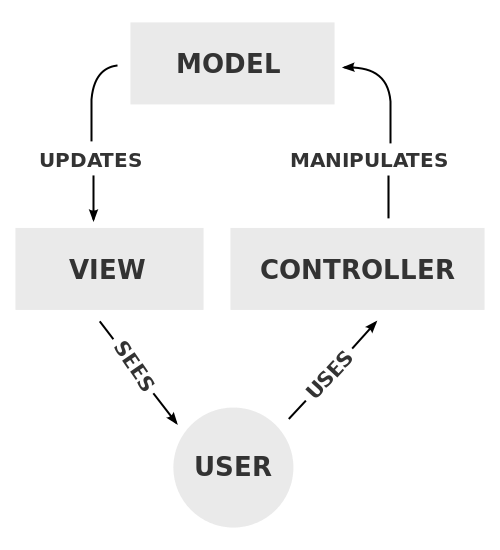
\includegraphics[height=55mm]{./img/mvc.png}
	\caption{Schemat wzorca projektowego Model View Controller}
	\label{fig:mvc-scheme}
\end{figure}


\section{Działanie frameworku}
ASP.NET MVC pozwala w łatwy oraz intuicyjny sposób obsługiwać żądania HTTP. W dużym skrócie działanie zostaje obsłużone w następujących krokach:
\begin{itemize}
\item Framework kieruje żądanie do odpowiedniego kontrolera na podstawie reguł routingu.
\item Kontroler generuje odpowiedź posługując się wybranym widokiem, do którego dostarcza spreparowane dane.
\item Dane pozyskiwane są przez klasy z warstwy modelu.
\item Silnik wypełnia widok danymi oraz zwraca odpowiedź w postaci kodu HTML.
\end{itemize}
MVC dostarcza również rozwiązań pozwalających na prosty dostęp do parametrów żądaniem, sesji, cookies oraz wiele innych. Mimo bogatej biblioteki oraz wymuszonej struktury projektu, programista posiada dużą swobodę tworząc aplikację.

\subsection{Struktura projektu}
Podczas tworzenia projektu MVC zalecane jest korzystane z domyślnej struktury projektu. W takim przypadku oprócz dobrej organizacji kodu, programista zyskuje wiele dodatkowych udogodnień takich jak uproszczone mechanizmy routingu, czy proste powiązanie kontrolera z widokiem. Nazwy folderów w intuicyjny sposób wskazują na to, co powinny zawierać. 

\begin{figure}[h]
	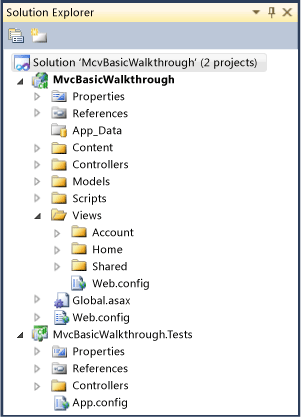
\includegraphics[height=55mm]{./img/mvc-project-structure.png}
	\caption{Struktura projektu ASP.NET MVC}
	\label{fig:mvc-project-structure}
\end{figure}

\subsection{Routing}
Najprostszym mechanizmem zarządzania routingiem w aplikacji jest trzymanie się konwencji nazewnictwa oraz umieszczania plików w odpowiednich folderach. Przykładowo url o postaci ,,http://localhost:8080/DeviceSchemes/EditScheme/20'' zostanie przekazany do kontrolera o nazwie \textit{DeviceSchemesController} i jego metody \textit{EditScheme}, która powinna posiadać jeden parametr. Parametry mogą zostać rzutowane na typy proste jak i na obiekty, co znacznie upraszcza obsługę złożonych obiektów JavaScript skonwertowanych do postaci JSON. 

Drugą częścią konfigurowania routingu jest korzystanie z metod obiektu RouteCollection. Reguły definiuje się określając wzór URLa, oraz kontroler i akcję, do których żądanie zostanie skierowane. Opcjonalnie można zdefiniować też parametry żądania, które zostaną powiązane z parametrami akcji kontrolera. Aby stworzyć powiązanie z poprzedniego przykładu, należy zdefiniować trasę w następujący sposób:

\begin{lstlisting}[language=Java]
routes.MapRoute("DeviceSchemes", "DeviceSchemes/EditScheme", 
	new { controller = "DeviceScheme", action = "EditScheme", schemeId})
);
\end{lstlisting}
Obiekt RouteCollection umożliwia także tworzenie bardziej uniwersalnych tras dzięki zastosowaniu nawiasów oraz słów kluczowych w URL. Przykładowo dodanie takiego routingu:
\begin{lstlisting}[language=Java]
routes.MapRoute(
    name: "Default",
    url: "{controller}/{action}/{id}",
    defaults: new { controller = "Main", action = "Index", id = UrlParameter.Optional }
);
\end{lstlisting}
spowoduje powiązanie każdego URL do kontrolera i akcji na podstawie nazewnictwa. W przypadku gdy kontroler i akcja o odpowiednich nazwach nie zostaną znalezione, żądanie zostanie przekierowane do domyślnego kontrolera \textit{MainController} oraz akcji \textit{Index}, której parametry są opcjonalne.
Podczas definiowania tras należy pamiętać, iż URL dopasowywany jest do reguł w kolejności ich definicji. Reguły należy zatem deklarować ze szczególną uwagą. Przykładowo, nie ma sensu dodawać reguł do tej samej akcji z różną liczbą parametrów w momencie gdy powyżej znajduje się deklaracja z parametrami opcjonalnymi. Należy również zwrócić uwagę na sytuację, w której powiązanie parametrów żądania z parametrami akcji jest niemożliwe. Dzieje się to, gdy typy parametrów są niezgodne i próba rzutowania kończy się wyrzuceniem wyjątku. Framework nie będzie kontynuował dopasowywania URL do kolejnych reguł.


\subsection{Warstwa kontrolerów}
Klasy będące kontrolerami powinny spełniać następujące założenia:
\begin{itemize}
\item Dziedziczyć po klasie Controller. 
\item Posiadać nazwę która kończy się słowem Controller (np. DeviceSchemesController).
\item Znajdować się w katalogu Controllers.
\end{itemize}
Wszystkie publiczne metody w kontrolerze nazywane są akcjami. W praktyce to właśnie one zawierają logikę biznesową, która obsługuje żądanie HTTP. Typ żądania z jakim powiązana zostanie akcja konfiguruje się za pomocą atrybutów (np. [HttPost] lub [HttpGet]). Rezultat działania akcji może znacznie różnić się w zależności od zwracanej przez niego wartości. Poniżej znajdują się niektóre z nich:
\begin{itemize}
\item View() - zwraca widok o nazwie odpowiadającej nazwie akcji, który musi znajdować się w katalogu o nazwie kontrolera. W przypadku kontrolera \textit{DeviceSchemesController} i akcji \textit{DevicesList} widok powinien nazywać się \textit{DevicesList} i znajdować się w katalogu o ścieżce \textit{Views/DeviceSchemes}.
\item View(,,nazwa widoku'') - działa jak wyżej z tą różnicą, iż zamiast nazwy domyślnej można podać jako parametr.
\item View(obiekt modelu) - tworzy tak zwany ,,typowany widok''. Szczegóły na jego temat znajdują się w następnym podrozdziale.
\item Redirect(,,url'') - przekierowuje na podany w parametrze adres.
\item RedirectToAction(,,nazwa akcji'', ,,nazwa kontrolera'', [opcjonalne parametry]) - pozwala przekierować żądanie do kolejnej akcji.
\item Json(obiekt) - konwertuje dany obiekt do postaci Json. Pozwala to na wygodną obsługę żądań asynchronicznych.
\end{itemize}
Wszystkie powyższe metody pomocnicze znajdują się w klasie Controller. Dzięki tej klasie możliwe jest również łatwe przesyłanie dowlonych obiektów do zwracanego z kontrolera widoku. Służą do tego obiekty ViewBag i ViewData. ViewData jest mapą, z której można korzystać w następujący sposób:
\begin{lstlisting}[language=Java]
ViewData["lastProjectId"] = lastProjectId;
int lastId = (int) ViewData["lastProjectId"];
\end{lstlisting}
Minusem mapy ViewData jest to, iż wszystkie wpisywane do niej obiekty są typu Object.
Inaczej jest w przypadku ViewBag, który jest dynamicznie tworzonym obiektem.  Obiekt ten utrzymuje typy przechowywanych danych, a korzystanie z niego wygląda następująco:
\begin{lstlisting}[language=Java]
ViewData.lastProjectId = lastProjectId;
int lastId = ViewData.lastProjectId;
\end{lstlisting}

\subsection{Przykładowy kontroler}
Poniżej znajduje się fragment przykładowego kontrolera.


\begin{lstlisting}[language=Java]
namespace Elements.Controllers
{
    public class DesignerController : Controller {
    
            [HttpPost]
            public ActionResult ProjectsList()
            {
                List<Project> projectsList;
                List<DeviceScheme> schemesList;
                using (var qm = new QueryManager())
                {
                    projectsList = qm.getAllProjects();
                    schemesList = qm.GetAllDevicesSchemes();
                }
                
                ProjectsListViewModel model = new ProjectsListViewModel();
                model.DeviceSchemes = schemesList;
                model.Projects = projectsList;
    			ViewBag.model = model;
    			
                return View(model);
            }
            
            ...     
    }
}
\end{lstlisting}


\subsection{Warstwa widoków}
Widokami nazywamy pliki z kodem HTML oraz wstawkami ASPX lub Razor. Służą one do prezentowania użytkownikowi danych spreparowanych przez kontroler. Widok powinien znajdować się w katalogu Views, podkatalogu o nazwie kontrolera, a sam nosić nazwę akcji. Dzieje się tak, gdyż z reguły każdy widok związany jest z określonym kontrolerem oraz akcją. 
Wstawki ASPX oraz Razor służą do dodawania dynamicznie wygenerowanej treści do widoków. Dzięki nim możliwe jest uzyskanie dostępu do klas pomocniczych oraz obiektów modeli (ViewBag, ViewData, Model) i sesji (Session). W powyższych wstawkach możliwe jest również korzystanie z kodu C\#, co umożliwia widokom posiadać logikę. Należy jednak pamiętać, że kod w widokach powinien służyć jedynie do prezentacji danych, a nie zastępować logiki biznesowej kontrolerów. Warto zauważyć, że kod zawarty we wstawkach wykonywany jest po stronie serwera w trakcie renderowania widoku. Do wykonywania działań w aplikacji po stronie klienta używana jest technologia JavaScript. Przykładowy fragment widoku z wykorzystaniem wstawek Razor wygląda następująco:

\begin{lstlisting}[language=HTML]
<div id="projectsContainer" class="boxContainer">
    <div class="header">
        <h1>Lista wizualizacji</h1>
    </div>
    <div class="content gradiendBackgroundGray">
        <div id="addProject" class="box addBox"><span>+</span></div>

        @foreach (var project in Model.Projects)
        {
            <div class="box projectBox boxGradientBackground" data-projectname="@project.Name" data-projectid="@project.Id">
                <button class="btn btn-danger actionButton removeButton"><span class="glyphicon glyphicon-remove"></span></button>
                <button class="btn btn-success actionButton updateButton"><span class="glyphicon glyphicon-pencil"></span></button>
                <h4 class="name">@project.Name</h4>
                <p><span class="bold">Grupa: </span><span class="deviceSchemeName">@project.DeviceScheme.Name</span></p>
                <p><span class="bold">Opis: </span><span class="description">@project.Description</span></p>
                <button class="btn btn-primary actionButtonBig viewProjectButton"><span class=" glyphicon glyphicon-search"></span></button>
            </div>
        }
    </div>
</div>
\end{lstlisting}

\subsection{Cykl życia aplikacji}
Rozdział ten zawiera krótki opis życia aplikacji ASP.NET MVC oraz jej składowych. Z punktu widzenia programisty są to bardzo istotne informacje, gdyż tworzenie obiektów klas definiowanych przez programistę często wykonywane jest przez framework. Aby mieć pełną kontrolę nad towrzoną aplikacją warto jest znać kolejne kroki podejmowane przez MVC podczas obsługi żądania HTTP.

W momencie gdy aplikacja jest uruchamiana na serwerze wywoływane są metody klasy MvcApplication, których zadaniem jest konfiguracja aplikacji. Klasa ta jest umieszczona w pliku Global.asax.cs. Pierwszą wywoływaną metodą klasy jest Application\_Start. Znajduje się w niej między innymi wywołanie wcześniej wspomnianej metody RegisterRoutes, w której definiuje się trasy routingu. W klasie MvcApplication można dodatkowo zdefiniować \textit{listenery} - metody, które zostają wywołane przez framework w momencie różnych zdarzeń podczas życia aplikacji. Mogą to być na przykład zdarzenia tworzenia oraz niszczenia sesji.
Od momentu odebrania żądania HTTP do zwrócenia użytkownikowi odpowiedzi framework wykonuje następujące czynności:
\begin{itemize}
\item URL zapytania zostaje porównane z definicjami tras.
\item W momencie, gdy zapytanie zostanie dopasowane do kontrolera i akcji framewrok tworzy obiekt odpowiedniej klasy kontrolera. 
\item Wywoływana jest odpowiednia akcja kontrolera. Gdy posiada ona parametry, są one przekazywane do akcji. Parametry są rzutowane na odpowiednie typy jeśli zachodzi taka potrzeba. W przypadku niepowodzenia rzutowania zostanie wyrzucony wyjątek.
\item W zależności od typu zwracanej wartości przez akcję, użytkownikowi użytkownikowi zwracana jest odpowiedź. Może to byc kod HTML, obiekt JSON lub pojedyncza wartość.
\end{itemize}

\begin{figure}[b]
	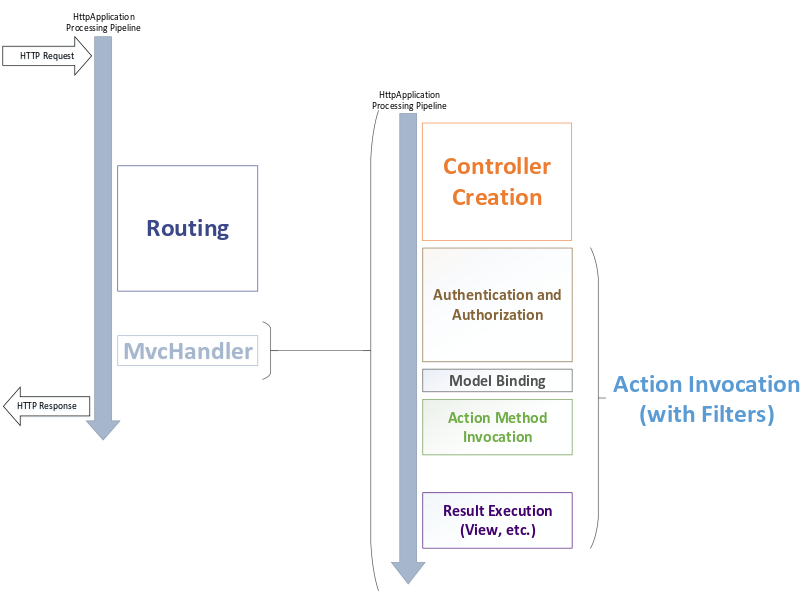
\includegraphics[width=140mm]{./img/mvc-diagram.png}
	\caption{Obsługa żądania HTTP}
	\label{fig:mvc-diagram}
\end{figure}




\subsection{Warstwa modeli}
Warstwa modeli zawiera wszystkie klasy, które opisują elementy składowe rozwiązywanego problemu. Warstwa ta powinna zawierać również mechanizmy pobierania oraz zapisu danych modeli. 
Framework pozostawia w tym miejscu programiście dużą swobodę działania. Nie ma narzuconej metody implementacji warstwy modeli. Jest to logiczne, gdyż aplikacja może pobierać i zapisywać dane na wiele sposobów, na przykład poprzez bazę danych, kolejki, pliki, itp. 
Przykładowa klasa należąca do warstwy może wyglądać następująco:
\begin{lstlisting}[language=Java]
public class DeviceScheme
{
        public int Id { get; set; }
        public string Name { get; set; }
        public string DevicesNames { get; set; }
        public IList<Project> Projects { get; set; }
}
\end{lstlisting}

\usetikzlibrary{trees}
\tikzstyle{every node}=[draw=black,thick,anchor=west]
\tikzstyle{module}=[draw=blue,fill=blue!30]
\tikzstyle{class}=[draw=green,fill=green!50]
\tikzstyle{function}=[draw=gray,fill=gray!50]
\tikzstyle{var}=[draw=orange,fill=orange!50]
\tikzstyle{interface}=[draw=purple,fill=purple!50]
\chapter{TypeScript}
JavaScript (JS) jest technologią, która od lat służy programistom do wzbogacania interfejsów stron internetowych o dynamikę\cite{javascript-book}. Dzisiaj JavaScript postrzegany jest jako technologia, która sprawia programistom wiele problemów. Wynika to przede wszystkim ze składni języka, braku mechanizmu typowania oraz uproszczonej metodzie tworzenia hierarchii klas \ref{fig:javascript-inheritance}. Efekt ten jest spowodowany faktem, iż w momencie powstawania języka JavaScript, panowało przeświadczenie, iż nie będzie służył on do tworzenia dużych, kompletnych aplikacji. Postawiono zatem na prostotę rozwiązania. Dzięki niej programista jest w stanie szybko osiągnąć zamierzony cel niewielką ilością kodu.

\begin{figure}[h]
	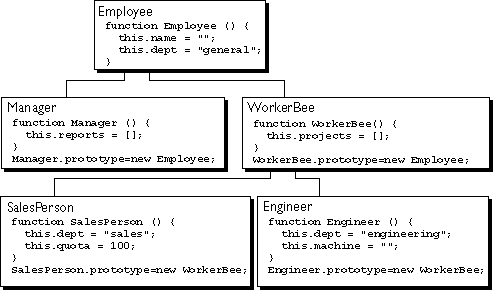
\includegraphics[width=140mm]{./img/javascript-inheritance.png}
	\centering
	\caption{Mechanizm dziedziczenia z wykorzystaniem obiektu prototype}
	\label{fig:javascript-inheritance}
\end{figure}

Rozwój aplikacji internetowych oraz przeglądarek pokazał, iż tworzenie bogatego interfejsu aplikacji daje wiele korzyści. JavaScript z biegiem lat nabierał znaczenia, gdyż coraz więcej przeglądarek wspierało tę technologię. W roku 1996 w oparciu o JS stworzony został standard o nazwie ECMAScript, który obsługiwany jest dziś przez wszystkie najpopularniejsze przeglądarki. 

Programowanie interfejsów aplikacji internetowych doszło zatem do punktu, w którym programiści zmuszeni są używać JavaScript do tworzenia dużych aplikacji\cite{javascript-book}. Stało się to pomimo faktu, iż technologia ta została zaprojektowana do innego celu. Odpowiedzią na ten problem jest język TypeScript autorstwa Microsoftu.

\section{Cechy technologii}
Technologia TypeScript (TS) składa się z dwóch elementów - języka oraz kompilatora. Oba z nich są projektami na licencji OpenSource dostępnymi dla każdego. Aby lepiej zrozumieć możliwości technologii należy zapoznać się z następującymi faktami na jej temat umieszczonymi poniżej.
\begin{itemize}
\item Język TypeScript jest kompilowany do języka JavaScript. Oznacza to, że poza kilkoma dodatkowymi słowami kluczowymi wystarczy znajomość JavaScriptu do posługiwania się TypeScriptem. 
\item Główną cechą TS rozszerzającą JS jest możliwość definiowania typów zmiennych. Poprawność typu sprawdzana jest przed kompilacją kodu TS do JS.
\item Każdy fragment kodu napisany w JavaScript może zostać użyty do rozwoju klas w języku TypeScript. Dzięki temu możliwe jest wykorzystywanie w projekcie TS popularnych bibliotek JS takich jak jQuery, MooTools, itp. Społeczność regularnie dostarcza pliki TypeScript, które zawierają definicje typów obiektów używanych przez różne biblioteki. Pozwala  to na wygodniejsze stosowanie ich zgodnie z zasadami języka TypeScript. 
\item Kompilator TypeScriptu zawarty jest w jednym pliku JavaScript i może zostać dołączony do każdego środowiska. Technologia nie posiada maszyny wirtualnej i nie ma planów na jej rozwój.
\end{itemize}

\section {Elementy składowe TypeScript}
Język programowania TypeScript został stworzony na podobieństwo języka C\#. Nazewnictwo oraz przeznaczenie elementów składowych języka są niemal identyczne.
Schemat programu wykonanego w technologii TypeScript wraz z jego elementami składowymi zobrazowany jest na poniższym rysunku:
\begin{figure}[h]
	\begin{tikzpicture}[%
	  grow via three points={one child at (0.5,-0.7) and
	  two children at (0.5,-0.7) and (0.5,-1.4)},
	  edge from parent path={(\tikzparentnode.south) |- (\tikzchildnode.west)}]
	  
	  \node {Program} 
	    child { node [module] {Moduł} {
	   		child { node [class] {Klasa} {
	   			child {node [var] {Zmienna}}}
	   	}	
	   		    child [missing] {}	
    	child { node [function] {Funkcja} {
    		child { node [var] {Zmienna}}}
    	}			
	    child [missing] {}	
    	child { node [interface] {Interfejs}}}
    	}
    	child [missing] {}	
    		   child [missing] {}	
    		   child [missing] {}	
    		   child [missing] {}	
    		   child [missing] {}	
    		   child { node [module] {Moduł} {
    		   	   		child { node [class] {Klasa} {
    		   	   			child {node [var] {Zmienna}}}
    		   	   	}	
    		   	   		    child [missing] {}	
    		       	child { node [function] {Funkcja} {
    		       		child { node [var] {Zmienna}}}
    		       	}			
    		   	    child [missing] {}	
    		       	child { node [interface] {Interfejs}}
    		   	    }};
    	
	\end{tikzpicture}
	
	\caption{Schemat wzorca projektowego Model View Controller}
	\label{fig:mvc-scheme}
\end{figure}

Przez pojęcie ,,program'' w technologii TypeScript rozumiemy zbiór plików źródłowych z rozszerzeniem \textit{.ts}. Pliki te mogą zawierać elementy opisane poniżej.
\begin{itemize}
\item Moduł - może zawierać wiele klas oraz interfejsów. Można o nich myśleć jak o namesace'ach w języku C\#.
\item Intefejs - wymusza na klasie posiadanie określonych metod o pól. W TypeScript'cie klasy mogą implementować wiele interfejsów. Interfejsy nie powodują generowania dodatkowego kodu JavaScript. Służą one do wymuszania przez kompilator na programiście zachowania zdefiniowanych kontraktów między klasami.
\item Klasa - posiada zmienne oraz funkcje. Dostępne są dwa modyfikatory dostępności funkcji - public oraz private. Klasa może dziedziczyć po jednej, innej klasie.
\item Funkcja - zawiera fragment logiki programu. Może przyjmować argumenty oraz zwracać wartość określonego typu lub void. Przykładowa deklaracja funkcji wygląda następująco:
\begin{lstlisting}[language=Java]
function getNumberString(parameter: number): string {
	return 'Podana liczba to: ' + parameter.toString();
}
\end{lstlisting}
\item Zmienna - może być określonego lub dowolnego typu. Dowolny typ należy oznaczać słowem kluczowym \textit{any}. Kontrola typów odbywa się na poziomie kompilatora, gdyż nie jest ona wymuszana przez JavaScript w trakcie wykonywania programu. Sprawdzenie typu przez kompilator odbywa się w przypadku przypisywania wartości do zmiennej i wywoływania funkcji. TypeScript posiada kilka wbudowanych typów. Są nimi:
\subitem number - 64-bitowa zmienna zmiennoprzecinkowa,
\subitem boolean - przyjmuje wartości true lub false,
\subitem string - sekwencja znaków UTF-16,
\subitem tablice - definiuje się je za pomocą nawiasów kwadratowych ,,[]'' lub za pomocą klasy \textit{Array}.
\end{itemize}

\section{Integracja TypeScript z istniejącym kodem JavaScript}
TypeScript umożliwia integrację z istniejącymi fragmentami kodu JS. Jest to przydatne w sytuacjach, gdy w TypeScript chcemy skorzystać ze zmiennych, które zdefiniowane się bezpośrednio w kodzie strony. Przykładowo:
\begin{lstlisting}[language=HTML]
	...
	<script type="text/javascript">
		var zewnetrznaZmienna = 10;
	</script>
	<script type="text/javascript" src="naszKod.js" />
	...
\end{lstlisting}

Aby w pliku \textit{naszKod} skorzystać ze zmiennej \textit{zewnetrznaZmienna} należy użyć słowa kluczowego \textit{declare}.
\begin{lstlisting}[language=Java]
	declare zewnetrznaZmienna : Number;
\end{lstlisting}

\subsection{TypeScript i jQuery}
Warto wspomnieć, iż w JavaScript możliwe jest przypisywanie do wskaźnika obiektu this dowolnej wartości. Niektóre biblioteki takie jak jQuery wykorzystują to, by ułatwić użytkownikowi manipulację elementami drzewa strony DOM. Dzieje się to na przykład podczas korzystania z metody \textit{each}:

\begin{lstlisting}[language=Java]
	$('.klasa').each(function(){
		$(this).attr('id', 'noweId');
	});
\end{lstlisting}
Powyższy kod iteruje po wszystkich węzłach o klasie ,,klasa'' i nadaje im nowe id. Dzięki temu, iż funkcja \textit{each} przypisuje wskaźnikowi \textit{this} wartość referencji do obiektu kolejnego iterowanego węzła, możliwe jest proste operowanie na jego parametrach. Jest to jednak kłopotliwe w przypadku języka TypeScript.

W poniższym przykładzie programista chciałby napisać metodę, która przypisze do pola obiektu wartość tekstową elementu o zadanym id. W tej sytuacji nie możliwe jest odniesienie się wewnątrz funkcji \textit{each} do pól / metod obiektu, gdyż wskaźnik \textit{this} został podmieniony.
\begin{lstlisting}[language=Java]
	class Finder{
		var nameToFind: String;
	
		public void findName(){
			$('.klasa').each(function(){
				if ((this).attr('id') == 'nazwa') {
					this.nameToFind = $(this).val(); //blad!
				}
			});
		}
	}
\end{lstlisting}

Twórcy technologii TypeScript dodali odpowiednią składnię do języka, która pomaga obejść ten problem. Wystarczy posłużyć się tak zwaną ,,arrow function'', która zwyczajnie zapisze wskaźnik \textit{this} do zmiennej pomocniczej \textit{\_this} przed wywołaniem metody w której jest on podmieniany, a następnie przywróci jego wartość po jej wykonaniu. Aby naprawić powyższy przykład należy dokonać takiej modyfikacji:

\begin{lstlisting}[language=Java]
	public void findName(){ () => {
		$('.klasa').each(function() {
			if ((this).attr('id') == 'nazwa') { 
					this.nameToFind = $(this).val(); //blad!
				}
			}
		});
	}
\end{lstlisting}

Skompilowany kod będzie miał następującą postać:
\begin{lstlisting}[language=Java]
	Finder.findName = function(){ 
		var _this = this;
		$('.klasa').each(function() {
			if ((this).attr('id') == 'nazwa') { 
					_this.nameToFind = $(this).val();
				}
			});
		this = _this;
		};
\end{lstlisting}

\chapter{Opis zastosowanego rozwiązania}

Rozdział ten zawiera opis zastosowanego w ramach pracy rozwiązania służącego do zdalnego nadzorowania pracy urządzeń. Rozwiązanie to zostało zaprojektowane dla dwóch typów użytkowników. Pierwszym z nich jest projektant widoków – osoba odpowiedzialna za ich tworzenie, która posiada podstawową wiedzę na temat urządzeń. Drugim typem użytkownika jest osoba upoważniona do oglądania widoków. W żargonie branży kolejowej termin ,,widok'' można zastąpić słowem ,,wizualizacja''.

Rozwiązanie zostało zaimplementowane jako aplikacja internetowa składająca się z dwóch modułów. Każdy z nich przeznaczony jest dla odpowiedniego typu użytkownika. Zadaniem pierwszego modułu aplikacji - ,,Elements Designer'' jest projektowanie widoków. Są to strony złożone z elementów graficznych, które pozwalają na wizualizację stanu urządzenia. Drugi moduł o nazwie ,,Elements Viewer'' służy do wyświetlania tych widoków wraz z nawiązaniem połączenia z urządzeniami i dostarczeniem danych w odpowiednie miejsca wizualizacji. Kolejne podrozdziały zawierają szczegółowy opis funkcjonalności modułów.

\section{Elements Designer - Moduł projektowania widoków}

Moduł Designer pozwala na projektowanie widoków urządzeń. Jego interfejs składa się z dwóch głównych elementów – menu bocznego oraz głównego obszaru roboczego, który prezentuje obecny stan projektu. Obszar ten nosi nazwę ,,sceny''. Dzięki temu rozwiązaniu projektant widzi efekt swojej pracy natychmiast po dokonaniu zmian.
Projektowanie widoku polega na wybieraniu tzw. komponentów z menu, umieszczaniu ich w odpowiednim miejscu na scenie i konfigurowaniu wedle potrzeb.

\subsection{Tworzenie projektu}

Po wybraniu modułu z odpowiedniej sekcji menu aplikacji użytkownikowi ukazuje się strona wyboru projektu. Każdy projekt widoczny jest jako kafelek z nazwą i opisem projektu. Użytkownik może z tego miejsca przejśc do edycji istniejącego projektu lub stworzyć nowy. W takiej sytuacji należy uzupełnić nazwę, opis oraz grupę urządzeń, dla której projektowany będzie widok. Po zatwierdzeniu tych danych użytkownikowi ukazuje się Scena.


\subsection{Scena}
Scena jest obszarem roboczym, który gromadzi wszystkie komponenty. Po zapisaniu projektu, możliwe będzie wyświetlenie jej przez moduł Viewer wraz ze wszystkimi komponentami naniesionymi na nią w trakcie projektowania. Jedynym atrybutem sceny, który można konfigurować jest kolor jej tła.

\subsection{Komponenty}
Komponenty to podstawowe elementy składowe projektu, które pełnią różne funkcje. W praktyce jest to każdy element dodany przez użytkownika do Sceny w trakcie projektowania. W aplikacji Elements istnieją trzy rodzaje komponentów, które można rozróżnić na podstawie ich funkcji:
\begin{itemize}
	\item Kontener – służy do grupowania innych komponentów. Można w nim umieścić dowolny komponent, ale sam również może być umieszczony w innym kontenerze. Aby umieścić element w kontenerze należy chwycić go myszą i ,,upuścić'' nad wybranym komponentem typu kontener. Czynność tę można odwrócić wybierając opcję ,,Przenieś wyżej'' z menu kontekstowego komponentu.
	\item TextBox – jego funkcja to przechowywanie tekstu, który można edytować. Dzięki temu możliwe jest tworzenie opisów innych elementów projektu. Tekst wpisywany jest podczas tworzenia komponentu. TextBox można edytować w każdej chwili wybierając odpowiednią opcję z jego menu kontekstowego.
	\item RefreshedVariable – element ten powiązany jest z konkretną zmienną urządzenia, którą należy wybrać podczas tworzenia komponentu. Jego główną funkcją jest regularne odświeżanie wartości zmiennej urządzenia w przypadku jej zmiany. Dodatkowo można skonfigurować zmianę tekstu i koloru tła komponentu w chwili gdy wartość zmiennej wyniesie lub przekroczy zdefiniowaną wartość. Pozwala to na zwrócenie uwagi użytkownika na zmienne w wyjątkowych sytuacjach. Można też ustawić komponentowi wartość domyślną. Dzięki temu komponent nie musi wcale zawierać liczby, a jedynie tekst informujący o stanie w jakim znajduje się urządzenie. Kolejną opcją jest nałożenie maski bitowej na zmienną. Przed wyświetleniem jej wartości element przemnoży ją przez liczbę ustawioną wcześniej jako maska. Jest to przydatne w przypadku gdy jedną zmienną należy interpretować jako więcej niż jedną liczbę. Ostatnią możliwością jest ustawienie wartości mnożnika. Komponent po prostu przemnoży wartość zmiennej przez mnożnik przed jej wyświetlaniem. W przypadku wybrania przez użytkownika opcji maski bitowej i mnożnika jednocześnie, mnożenie wykonywane jest jako ostatnia operacja.
\end{itemize}

Wszystkie komponenty posiadają dodatkowo kilka wspólnych właściwości, które można konfigurować wedle upodobań. Są nimi kolor tła, kolor obramowania, współrzędne oraz rozmiar. Wszystkie wyżej wspomniane właściwości można zmienić w dowolnej chwili posługując się menu kontekstowym dostępnym pod prawym przyciskiem myszy.  Dla wygody użytkownika rozmieszczenie komponentu określa się przeciągając go po scenie z miejsca na miejsce. Rozmiar natomiast reguluje się chwytając za wybrany narożnik komponentu i rozciągając go.

W momencie gdy użytkownik uzna iż projekt jest już gotowy musi go zapisać, aby zmiany nie zostały utracone. Służy do tego guzik z ikoną dyskietki znajdujący się w menu bocznym. Do edycji można wrócić w każdej chwili wybierając projekt ponownie z listy projektów.


\section{Elements Viewer – moduł wyświetlania widoków}
Moduł Viewer służy do prezentowania widoków użytkownikom końcowym – głównie kolejarzom. Viewer jest w stanie wczytać projekt widoku i wyświetlić go użytkownikowi utrzymując przy tym połączenie z urządzeniami i wyświetlając ich zmienne w skonfigurowany przez projektanta sposób.

\subsection{Lista urządzeń}
Pierwszą stroną, która ukazuje się użytkownikowi po uruchomieniu modułu jest lista wszystkich urządzeń podłączonych do aplikacji Elements. Konfiguruje się ją edytując odpowiedni plik xml w folderze aplikacji. Każde urządzenie na liście reprezentowane jest przez pojedynczy kafelek, który wyświetla jego nazwę. Po kliknięciu na guzik z ikoną lupy użytkownik zostaje przeniesiony do listy projektów dostępnych dla urządzenia.

\subsection{Lista projektów}
Interfejs listy projektów prezentuje się analogicznie do listy urządzeń. Każdy projekt reprezentowany jest przez kafelek z jego nazwą i opisem. Aplikacja przyporządkowuje widoki do urządzeń na podstawie przynależności urządzenia do grupy. Oznacza to, że wiele urządzeń może zostać przeniesionych do tego samego widoku, który wyświetli w nim zmienne wybranego urządzenia.

\subsection{Wizualizacje pracy urządzeń}
Głównym elementem widocznym na stronie projektu jest Scena. Wygląda ona prawie identycznie jak w module Designer. Różnica polega na tym, że menu projektowania jest ukryte. Użytkownik nie może też przesuwać komponentów ani wywołać menu kontekstowego. Widok jest przeznaczony jedynie do oglądania.
	
Po wybraniu projektu użytkownikowi ukazuje się układ komponentów wraz z nadanymi im atrybutami przez projektanta. Aplikacja nawiązuje połączenie z serwerem wymiany danych z urządzeniami w celu uzyskania wartości zmiennych dla komponentów typu RefreshedVariable. Połączenie z serwerem utrzymywane jest przez cały czas, gdy użytkownik znajduje się na stronie projektu. Dzieje się tak, ponieważ aplikacja regularnie kontroluje, czy wartości zmiennych nie uległy zmianie i w takim przypadku aktualizuje je w komponentach. Aktualizacja zmiennej polega na wyświetleniu jej w komponencie RefreshedVariable, który jej z nią związany. Przed wyświetleniem zmiennej aplikacja wykonuje dodatkowe czynności, uwzględniając konfigurację danego komponentu przez projektanta (zmiana tekstu, zmiana koloru, maska bitowa, mnożnik).
\chapter{Implementacja}

Aplikacja Elements została zaprojektowana w taki sposób, by z łatwością można było ją dopasować do innych składowych systemu ogrzewania rozjazdów kolejowych. W związku z tym, aplikacja przygotowana jest do instalacji na serwerze xsp4 zintegrowanym z apache, przy użyciu maszyny wirtualnej Mono. Wyżej wymienione technologie są kompatybilne z systemami z rodziny Unix, na których działa reszta aplikacji systemu.

\section{Wykorzystane biblioteki}

\subsection{Razor}

Razor jest silnikiem generowania widoków autorstwa Microsoft, który w swojej składni jest znacznie prostszy niż jego poprzednik – aspx. Dzięki temu tworzenie stron, które wymagają użycia logiki staje się jeszcze łatwiejsze. Uproszczenie składni polega głównie na zastąpieniu znaczników aspx jednym znakiem - „@”. Służy on do zadeklarowania w widoku intencji użycia zmiennych dostarczanych do niego przez kontroler. Wydawać by się mogło, że nie jest to duża różnica, lecz w przypadku skomplikowanych konstrukcjach warunkowych łatwo dostrzec przewagę silnika Razor nad aspx. Dla przykładu następującą składnię aspx:

\begin{lstlisting}[language=HTML]
<%if (Model.Length == 0)

       else
 {%>
   <p><%=Model.Item%></p>
<%} %>
\end{lstlisting}
można zastąpić w taki sposób:
\begin{lstlisting}[language=HTML]
@if (Model.Length == 0)
{
        <p>Brak</p>
}
 else
{
        <p>@Model.Item</p>
}
\end{lstlisting}
W widoku można umieścić sekcję zawierającą logikę. W tym celu należy umieścić linie kodu w konstrukcji @\{...\}. Warto jednak nie zapominać o podstawowym założeniu MVC – widok powinien wyświetlać dane, a nie służyć do ich generowania \cite{design-patterns}.
Razor zawiera również prosty mechanizm tworzenia szablonów stron. Dzięki temu ilość kodu w plikach widoków znacznie się zmniejsza, gdyż powtarzalne części strony takie jak menu, czy stopka można wyeksportować do odrębnych plików.

\subsection{NHibernate}
Nhibernate jest biblioteką, która służy do powiązania tabel baz danych na obiekty (Object Related Mapping) \cite{nhibernate-doc}. Dzięki niej możliwe jest posługiwanie się prostymi obiektami, które swoją strukturą odpowiadają odpowiednim tabelom. Dużą zaletą NHibernate w stosunku do innych bibliotek spełniających tę funkcję jest możliwość konfiguracji w kodzie. Skonfigurować w kodzie można zarówno sposób wiązania obiektów z tabelami, jak i samo połączenie z bazą. Najprostszą metodą konfiguracji jest wskazanie, w którym pakiecie znajdują się obiekty, które powinny zostać powiązane z tabelami za pomocą klasy Configuration. Należy jedynie pamiętać, by nazwy obiektów oraz ich pól były identyczne jak odpowiednie nazwy tabel oraz ich kolumn. Dzięki klasie Configuration uzyskujemy dostęp do obiektu typu SessionFactory, który pozwala na otwieranie i zamykanie sesji z bazą danych. 

Kolejną zaletą NHibernate jest możliwość wykorzystania technologii LINQ do wykonywania zapytań. Dzięki temu kod C\# zawierający zapytanie jest bardzo podobny do odpowiadającego mu zapytania SQL i naturalnie opisuje intencje programisty. Na przykład zapytanie SQL o postaci:
\begin{lstlisting}[language=SQL]
SELECT
    Name
FROM
    Device
WHERE
    Id = 1;
\end{lstlisting}
można zapisać w następujący sposób:
\begin{lstlisting}[language=Java]
string name = session.QueryOver<Device>()
    .Where(d => d.Id == 1)
    .Select(d => d.Name)
    .SingleOrDefault<string>();
\end{lstlisting}
Używanie biblioteki opiera się głównie na wykorzystaniu obiektu SessionFactory. Służy on do otwierania połączenia z bazą danych, wykonywania operacji oraz zamykania połączenia. Wszystkimi wymienionymi czynnościami zajmuje się biblioteka, pozwalając programiście skupić się na logice biznesowej programu.

\subsection{jQuery}
jQuery to biblioteka, która pozwala na osiąganie atrakcyjnych efektów wizualnych na stronie WWW niewielkim nakładem pracy programisty. Jak wiadomo z dokumentacji \cite{jquery-doc}, całość wykonana jest w oparciu o technologię JavaScript. Biblioteka jest niezależna od przeglądarki więc programista nie musi dostosowywać kodu do wielu różnych przeglądarek WWW. Korzystanie z biblioteki polega głównie na korzystaniu z obiektu jQuery lub znaku "\$", który jest aliasem do tego obiektu. jQuery umożliwia wybieranie tablicy węzłów DOM strony internetowej, a następnie wykonywanie na nich różnych działań za pomocą języka JavaScript. Wybieranie węzłów wykonuje się wykorzystując selektory języka CSS3. Przykładowe działania to:
\begin{itemize}
\item dodawanie, usuwanie węzłów
\item odczytywanie i modyfikowanie atrybutów i zawartości węzłów
\item modyfikowanie stylu węzłów
\item animacje
\item rozbudowana obsługa zdarzeń takich jak kliknięcie lub przesunięcie kursora nad element
\end{itemize}
Wszystko to można osiągnąc za pomocą kilku linii kodu, na przykład jeśli programista chciałby zmienić kolor tekstu wszystkich węzłów o klasie ,,red'', wystarczy posłużyć się następującym kodem:
\begin{lstlisting}[language=Java]
$('.red').css('color': 'red')
\end{lstlisting}
Kolejną istotną funkcją jQuery z punktu widzenia mojej aplikacji jest możliwość wykonywania zapytań synchronicznych jak i asynchronicznych AJAX. Znacznie przyspiesza to tworzenie aplikacji, gdyż różne przeglądarki wymagają obsługi wyżej wymienionych zapytań na różne sposoby. 

W internecie dostępnych jest wiele wtyczek do biblioteki, które rozszerzają funkcjonalność jQuery. Dzięki nim można na przykład w szybki sposób tworzyć interaktywne tabele z danymi (DataTables), przybornik do wyboru koloru (Evol), czy efektywny pokaz slajdów (Fotorama).

\section{Architektura aplikacji}
Zastosowane rozwiązane zostało zaimplementowane jako aplikacja internetowa. Moduł Viewer ma za zadanie wyświetlanie stanu urządzeń w przeglądarce internetowej. Drugi z modułów służy do projektowania tych widoków. Aby maksymalnie ułatwić użytkownikowi tę czynność, moduł Designer został zrealizowany w ten sam sposób. Dzięki temu projektant widoków ma natychmiastową możliwość oceny rezultatów swojej interakcji z aplikacją. Aplikacja została nazwana ,,Elements''. Nawiązuje to do małych elementów, z których budowane są widoki. 

Architektura projektu Elements składa się z trzech warstw zgodnie z ideą wzorca projektowego MVC. Jest to wymuszone przez framework ASP.NET MVC4. 

\subsection{Warstwa prezentacji - Widoki}
Warstwą prezentacji (View) jest interfejs graficzny modułów Designer oraz Viewer. Został on wykonany w dwóch technologiach. Strony internetowe budowane są za pomocą silnika tworzenia widoków Razor. Widoki te zawierają również logikę napisaną w języku TypeScript, który kompiluje się do kodu Javascript. Dzięki temu połączeniu użytkownik jest w stanie poruszać się po interfejsie aplikacji w płynny sposób. Nie ma konieczności przeładowywania formularza na stronach z każdą jego akcją dzięki zastosowaniu zapytań asynchronicznych AJAX. Właśnie na nich oparty w większości jest moduł Viewer. Moduł regularnie wysyła zapytania asynchroniczne do serwera aplikacji w celu pozyskania aktualnych zmiennych. W ten sposób osiągnięty został efekt monitorowania urządzeń w czasie rzeczywistym.

\begin{figure}[h]
	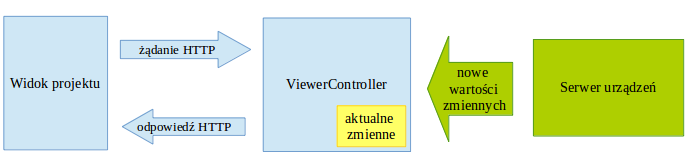
\includegraphics[width=150mm]{./img/viewer.png}
	\caption{Mechanizm odświeżania wartości zmiennych urządzeń}
	\label{fig:viewer}
\end{figure}

Komponenty zostały zaimplementowane za pomocą klas TypeScript. Klasy reprezentujące komponent dziedziczą po klasie Component oraz implementują któryś z interfejsów - Container, TextBox, RefreshedVariable, w zależności od ich przeznaczenia. Dzięki temu aplikacja może za pomocą jednego mechanizmu wyświetlić każdy komponent, zachowując przy tym jego specyficzne zachowanie. Scena jest wyjątkowym komponentem typu kontener. W module Designer pozwala to na przechowywanie komponentów, organizując je w strukturę drzewa. W module Viewer Scena regularnie odświeża zmienne w posiadanych komponentach typu RefreshedVariable. Dzieje się to w następujący sposób:
\begin{itemize}
\item scena iteruje po drzewie komponentów, które zawiera i gromadzi listę zmiennych związanych z elementami typu RefreshedVariable,
\item wysyłane jest zapytanie asynchroniczne z listą zmiennych w celu pozyskania ich,
\item po odebraniu odpowiedzi z serwera Scena iteruje po swoich komponentach i powiadamia je o zdarzeniu przybycia zmiennej,
\item Każdy komponent reaguje na przyjście nowej zmiennej w sposób wcześniej skonfigurowany przez projektanta widoków. Wykorzystany został tutaj wzorzec projektowy Observer-Observable.
\end{itemize}

Komponenty są zdolne do reagowania na zdarzenie przyjścia nowej zmiennej dzięki posiadanych przez nie list tzw. działań (rodzina klas dziedzicząca po klasie Behavior). W momencie przyjścia odpowiedzi z serwera zawierającej zmienne, Scena przekazuje ich wartości do odpowiednich komponentów. Komponenty te uruchamiają metody posiadanych działań, które sprawdzają czy wartość zmiennej spełnia warunek wykonania akcji np. czy wartość zmiennej jest większa od nadanej przez projektanta wartości. Jeśli tak jest, działanie modyfikuje odpowiednie pola komponentu zmieniając np. jego kolor lub tekst. Taki model klas nazywany jest wzorcem projektowym Dekorator. 
W Elements zostały zaimplementowane następujące zachowania:
\begin{itemize}
\item ColorChangeBehavior - zmienia kolor komponentu
\item TextChangeBehavior - zmienia tekst komponentu
\item ValueChangeBehavior - zmienia wartość numeryczną komponentu - każdy komponent domyślnie posiada to zachowanie
\end{itemize}
Do komponentu można dodać wiele zachowań jednocześnie. W takim przypadku kolejność zmian atrybutów komponentów jest zależna od kolejności dodania zachowania.

\subsection{Warstwa logiki biznesowej - Kontrolery}
Do warstwy logiki biznesowej w Elements należy część aplikacji wykonana w języku C\#, która wykonywana jest przez serwer aplikacyjny. Logika warstwy zawarta jest w tzw. kontrolerach - klasach, których zadaniem jest odbiór żądania HTTP od warstwy prezentacji i odesłania jej odpowiedzi. Odpowiedzią może być odpowiednio spreparowany widok lub pojedyncza wartość. Jako że aplikacja Elements jest oparta w dużej mierze na zapytaniach asynchronicznych, zadaniem każdego kontrolera jest dostarczenie odpowiedniego widoku oraz obsługa jego zapytań AJAX.

Głównym zadaniem kontrolera modułu Designer (klasa DesignerControler) jest dostarczanie widoków do tworzenia, usuwania i edytowania projektów. Zapis projektu odbywa się poprzez serializację klasy JSONProject dostarczanej z widoku, która zawiera drzewo komponentów, nazwę oraz opis projektu. Kontroler jest w stanie zapisać tę klasę do pliku jak i do bazy danych. Przesłanie projektu do widoku wykonane jest analogicznie, poprzez pobranie danych o projekcie z bazy i przesłanie ich do widoku w postaci obiektu klasy JSONProject. 

Kontroler modułu Viewer (ViewerController) odpowiada za dostarczenie widoków prezentujących listę projektów oraz wyświetlających ich zawartość. Projekty przesyłane są do widoku w taki sam sposób jak opisano powyżej. Głównym zadaniem kontrolera jest dostarczanie zmiennych do widoku projektu. Utrzymuje on stałe połączenie z serwerem urządzeń. Dzięki protokołowi wymiany danych DIMNET-P5, serwer urządzeń powiadamia kontroler o nadejściu nowych zmiennych oraz umożliwia natychmiastowe pobranie ich. Wartości zmiennych przechowywane są w słownikowej strukturze danych, która dodatkowo zawiera informacje o tym, czy określona zmienna zmieniła się od ostatniej aktualizacji widoku. Aby maksymalnie zwiększyć szybkość odświeżania wszystkich zmiennych widoku, kontroler przesyła do widoku jedynie te zmienne, które zmieniły swoje wartości od ostatniej aktualizacji.

Pozostałe kontrolery (klasy DeviceSchemesControler, MainControler) zajmują się tworzeniem i edycją grup urządzeń zapisywanych do bazy danych oraz nawigacją po aplikacji.

\subsection{Warstwa obsługi danych - Modele}
Aplikacja Elements zawiera dwa rodzaje modeli opisane poniżej.
\begin{itemize}
\item Pasywne - wszystkie klasy po stronie serwera zaimplementowane w tehcnologii C\#. Służą one głównie do przesyłu danych z widoku do kontrolera oraz do komunikacji z bazą danych. Potrzebne jedynie do reprezentacji fragmentów realizowanego projektu. Nie zmieniają same swojego stanu, gdyż nie posiadają one żadnej logiki. 
\item Aktywne - zaimplementowane w technologii TypeScript. Służą do reprezentacji graficznych elementów interfejsu użytkownika np. scena, komponenty lub urządzenia. Są w stanie zmieniać swój stan, odświeżając przy tym interfejs.
\end{itemize}

Do przechowywania danych została użyta baza PostgreSQL. Wynika to z faktu, iż jest ona już wykorzystywana w istniejącym systemie ogrzewania i oświetlania rozjazdów. Dodatkowymi atutami bazy PostgreSQL są: \cite{postgresql-book}
\begin{itemize}
\item konkurencyjna wydajność
\item bogata w typy danych
\item dojrzałość projektu, duża społeczność
\end{itemize}


\chapter{Podsumowanie}

\section{Cel projektu}
Zadaniem niniejszej pracy magisterskiej było zaprojektowanie oraz wykonanie narzędzia służącego do generowania stron internetowych w celu zdalnego monitorowania urządzeń energetyki kolejowej. Stworzona aplikacja została nazwana ,,Elements''. Narzędzie to miało przede wszystkim zaprezentować nową formę monitoringu urządzeń elektrycznych polegającą na dostarczaniu danych ze sterowników w czasie rzeczywistym. Jest to alternatywa dla obecnego rozwiązania o nazwie System Monitoringu Urządzeń Eleketrycznych (SMUE), które opiera się na danych archiwalnych przesłanych do serwera. Skutkiem takiej architektury systemu jest brak możliwości reagowania na nagłe zdarzenia, takie jak usterki oraz alarmy pożarowe i antywłamaniowe. Elements rozwiązuje ten problem dostarczając następujących funkcjonalności:
\begin{itemize}
\item pozwala projektować oraz prezentować projekty wizualizacji pracy urządzeń w oknie przeglądarki internetowej,
\item dane z urządzeń wyświetlane są w czasie rzeczywistym; czas transportu danych z urządzeń do momentu wyświetlenia ich w przeglądarce nie przekracza dwóch sekund,
\item dane wizualizacji odświeżają się automatycznie,
\item do projektowania wizualizacji nie jest wymagana szczegółowa wiedza na temat budowy urządzeń.
\end{itemize}


\section{Wyniki projektu}
Projekt Elements został zrealizowany jako aplikacja internetowa. W jego skład wchodzą dwa moduły. Pierwszym z nich jest Designer. Służy on do projektowania widoków wizualizacji za pomocą tak zwanych komponentów podzielonych z uwagi na pełnioną funkcję. Do jego obsługi wymagana jest podstawowa wiedza na temat budowy urządzeń grzewczych. Drugim modułem aplikacji jest Viewer, odpowiedzialny za prezentowanie wcześniej stworzonych widoków. Do jego obsługi nie jest wymagana specjalistyczna wiedza.

Warstwa serwera aplikacji wykonana została w technologii ASP.NET MVC 4. Jako silnik generujący dynamiczną treść stron użyty został Razor. 

Do realizacji warstwy interfejsu użytkownika posłużono się technologią TypeScript oraz bibliotekami BackboneJS i jQuery. Umożliwiło to proste wykonanie dość dużych wymagań względem interfejsu.

Elements jest przystosowany do wdrożenia zarówno na maszynach z systemem Windows, jak i Linux. Należy pamiętać, że w przypadku Linuxa, konieczne będzie wykorzystanie maszyny wirtualnej \textit{Mono}.

Projekt był testowany w firmie Arex jako prototyp nowego sposobu monitoringu urządzeń firmy. Aplikacja osadzona została na serwerze w systemie Linux. Do testów wykorzystano kilka urządzeń działających w terenie podłączonych do serwera danych. Testy polegały na tworzeniu wizualizacji, a następnie włączaniu ich na wiele godzin i monitorowania zmian w urządzeniach. Ustalony został limit przekroczenia czasu (2s.) dostawy danych od momentu żądania, który nie mógł zostać przekroczony przez aplikację. Wymaganie to zostało spełnione. Można zatem stwierdzić, iż oczekiwania względem projektu zostały zrealizowane. W chwili zakończenia pisania niniejszej pracy aplikacja Elements nie jest rozwijana. Plany na jej dalszy rozwój nie są znane.



\singlespacing
\bibliography{bibliography}
\bibliographystyle{unsrt}
\addcontentsline{toc}{chapter}{Bibliografia}
\listoffigures
\addcontentsline{toc}{chapter}{List of Figures}
\listoftables
\addcontentsline{toc}{chapter}{List of Tables}
\onehalfspacing

%\begin{appendices}

%\chapter{Title of Appendix A}

Appendices should be consecutively denoted with letters of the alphabet. An Appendix should include necessary supplementary data, e.g. calculations or schematic diagrams.
%\chapter[]{Title of Appendix B}

Detailed guidelines regarding the content of Appendices should be established by the faculty, taking into account the specificity of a given field and course of study.

%\end{appendices}

\end{document}
